\chapter{Mathematical model of the proposed triangulation}
\label{chap2}

Ordered set $V, E, F$, where $V$ is the set of vertices, $E$ is the set of edges given
by two vertices and $F$ is a set of faces given by three vertices is called triangular
mesh.

The triangulation of a surface is an approximation of the surface by a triangular mesh.

A correct triangulation shoud approximate the surface precisely enough and
be topologically equivalent to the surface. Moreover, a quality triangulation
should have triangles as equilateral as possible and adapt the size of the triangles
to the local curvature of the surface.

Two of the best known approaches when triangulating the implicit surface are
Marching Cubes \cite{lorensen1987marching} and Marching Triangles \cite{hilton1996marching}.
While Marching Cubes is a fast algorithm producing non-quality mesh, the Marching triangles
produces quality mesh for the cost of slower algorithm runtime.



\section{Triangulation adaptive to the local curvature}
\label{sub3.1}

As we explained at the beginning of chapter~\ref{sub2.1}, the curvature of a surface
measures how much the surface bends.

The triangulation of the surface should be accurate enough but also memory efficient.
It can be achieved by creating a triangulation which is locally adaptive to the
curvature of the surface. Therefore, having smaller triangles where
the surface is curved and bigger triangles where the surface is flatter.

In this section, we present our implementation of the triangulation adaptive
to the local curvature.

In the original algorithm, the height of the triangle which is projected
to the surface is set to the constant value $\frac{\sqrt{3}}{2}e$, where $e$ 
is the required length of the side of the triangle. To achieve the adaptivity
of the size of the triangles, we set the height of the triangle to depend on the curvature in
the given point, as shown in the Figure~\ref{img:15}.

\begin{figure}
    \centerline{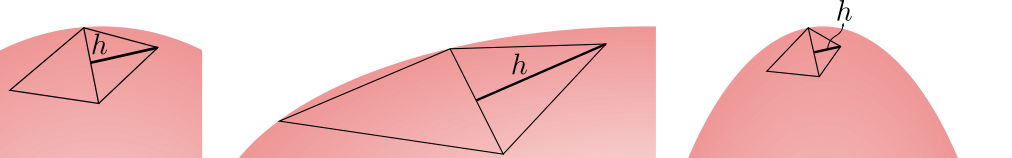
\includegraphics[scale=0.5]{images/img15}}
    \caption[Adaptive height of the new triangle]
    {Adaptive height of the new triangle.}
    %id obrazku, pomocou ktoreho sa budeme na obrazok odvolavat
    \label{img:15}
\end{figure}

To identify the curved areas, we decided to use the curvedness defined by 
Koendering and Doorn in 1992 \cite{koenderink1992surface}. As the authors 
explained, the Gaussian curvature and the mean curvature are not very descriptive
of the local shape of the surface. Principal curvatures taken as a pair
are more informative. The curvedness was introduced to measure 
the curvature in the given point by a single number instead of a
pair of numbers. The authors defined curvedness as 
$$c=\sqrt{\frac{\kappa_1^2+\kappa_2^2}{2}},$$
where $\kappa_1$ and $\kappa_2$ are the principal curvatures in the given point.

Curvedness has some obvious properties:
\begin{itemize}
    \item if $\kappa_1 == \pm\kappa_2$, then $c=|\kappa_1|=|\kappa_2|$,
    \item if $|\kappa_1|<|\kappa_2|$, then $|\kappa_1|<c<|\kappa_2|$,
    \item $c=0$ only in planar points,
    \item $c\geq0$. 
\end{itemize}

One could say that curvedness says only about the amount of the curvature
in the given point, not about the way the surface is curved at that point.

As an example, we describe the curvedness of the sphere and cylinder:
\begin{itemize}
    \item \textbf{Sphere:} As the principal curvatures of a sphere are both 
    equal to the inverse of the radius of the sphere, curvedness is also equal 
    to the inverse of the radius of the sphere.
    \item \textbf{Cylinder:} One of the principal curvatures of a cylinder
    is equal to zero, and the other is equal to the inverse of the radius of 
    the cylinder, curvedness is therefore equal to half of the inverse of 
    the radius of the cylinder.
\end{itemize}
 
Let us define the curvedness radius as $r_c = \frac{1}{c}$. It can be perceived as
the radius of a sphere, with curvedness $c$.

For the triangulation adaptive to the local curvature of the surface, an input
size of the edge $e$ is not perceived as the approximate size of the triangulation
triangle. Instead, it is perceived as a measure of the level of detail.
For the given edge size $e$, the level of detail for the triangulated surface
is the same as if we wanted to triangulate the unit sphere uniformly using
the triangles with the edge size $e$.

Let us define the constant of detail as $k_d = \frac{1}{e}$. It can be perceived
as the number of times the edge size $e$ would fit into the radius of the unit
sphere.

Then, for given point $P$, lying on the surface, the size of the edge, which
should be used around that point to achieve the desired detail, is 
calculated as the size of the edge which would fit $k_d$--times int $r_c$.
A maximum edge size is set to avoid the edge case in the planar point.

During the algorithm, for a given edge $E$ with the length $l_E$, the point
$C$ is created as displayed on the Figure~\ref{img:57}. The point $C$ lies
in the plane of the incident triangle of the edge $E$ on the line perpendicular
to $E$ and passing through $M_E$--midpoint of the edge $E$. The distance between
$M_E$ and $C$ is the height of the equilateral triangle with the edge $E$.

The curvedness is computed in each of the points $A$, $B$ and $C$.
The maximal value of the three computed values is used.
To avoid fast changes of the triangle size, some constraints are 
introduced. 

Inspired by the article by Akkouche and Galin \cite{akkouche2001adaptive},
let us define $l_{avg}$ as the average length of the set of edges consisting
of the edges incident with the points $A$ and $B$ on the boundary of the mesh
and the edge $E$.
The rate at which the triangle height can scale compared to
the height of the equilateral triangle with the edge length $l_{avg}$ is set to 30\%. 

\begin{figure}
    \centerline{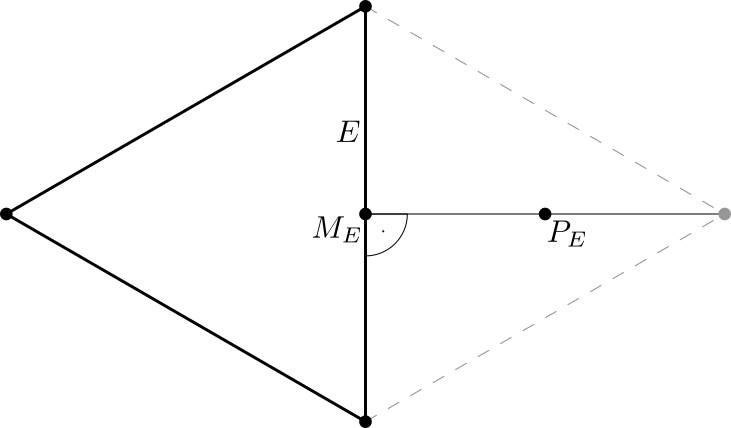
\includegraphics[scale=0.5]{images/img57}}
    \caption[Creating the point $C$]
    {Creating the point $C$ for the given edge $E$.}
    %id obrazku, pomocou ktoreho sa budeme na obrazok odvolavat
    \label{img:57}
\end{figure}

We calculate the edge length for the given constant of detail as $\frac{r_c}{k_d}$
which is equal to $\frac{e}{c}$, where $e$ is the size of the edge on the input 
and $c$ is curvedness in the point $P_E$. The new point is then created on the same
line perpendicular to the edge $E$ in the distance $\frac{\sqrt{3}e}{2c}$ from the point
$M_E$.

The result of the adaptive triangulation is best visible on a torus, as the curvedness
of the torus is maximal in the inner part of the torus and minimal in the outer part of the torus.
The resulting mesh for four different constants of detail for a torus is displayed on the
Figure~\ref{img:58} in the top row. One may note the difference in the sizes of the 
triangles in the inner
part of the torus and the outer part of the torus.

\begin{figure}[h!]
    \centerline{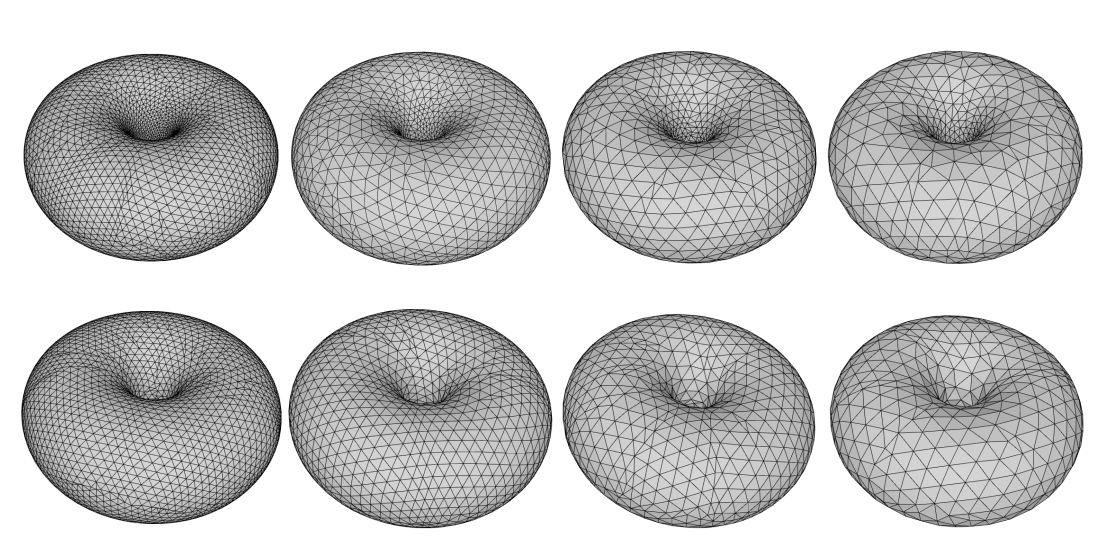
\includegraphics[scale=0.5]{images/img58}}
    \caption[Adaptive triangulation of a torus]
    {Adaptive triangulation of a torus with four different constants of detail (top row).
    Uniform triangulation of a torus with four different constants of detail (bottom row).}
    %id obrazku, pomocou ktoreho sa budeme na obrazok odvolavat
    \label{img:58}
\end{figure}

In contrast, the uniform triangulation of the same torus for four different edge lengths
is displayed in the bottom row in the Figure~\ref{img:58}. One may note that the 
triangles in the inner part of the torus are approximately the same 
size as those in the outer part.

\section{Triangulation of ADE singularities}
\label{sub3.2}

\subsection{Analysis of the geometry of ADE singularities}

ADE singularities are simple, isolated surface singularities which can be
expressed by corresponding implicit equations.

We already know that $A_{1--}$ singularity is locally represented as a cone.
This section discusses the geometric structure of other ADE surface singularities.

\begin{definition}
    Let us define the branch of ADE singularity as the part of the implicit surface
    connected to the rest of the implicit surface only by the singular point.
\end{definition}

\begin{comment}
\begin{definition}
    Let us define the triangulation direction of ADE singularity $A$ with radius $r$ as
    a direction $\vec{v}$ for which 
    $$F\bigg(A+t \vec{v} \cap S_{r}(A)\bigg) < 0,$$
    where $F$ is the implicit equation defining the singularity $A$
    and $t,r \in \R^+$.
\end{definition}
As we can see, each ADE singularity has infinitely many triangulation directions.
\end{comment}

For our needs, we pick one triangulation vector for each branch of
each ADE singularity. This triangulation vector is a normalized vector
either in the direction
of the rotation symmetry axis or an intersection of reflection symmetry planes
of the corresponding branch. If the branch has only one reflection symmetry
plane, the triangulation vector is picked to lie in the reflection
symmetry plane.

\begin{comment}
Moreover, when placed at the singular point, the triangulation vector of a branch 
is in the same half-space as the corresponding branch.
\end{comment}

In the general case, triangulation vectors serve us
as partial information about the orientation of a singularity with 
respect to its normal form.

\subsubsection*{$A_n$ singularities}

As we can see from the equations 
$F(x,y,z)=x^{n+1}\pm y^2\pm z^2$, $A_{n-+}$
singularities are just rotated $A_{n+-}$ singularities and $A_{n++}$ singularities 
are a single point if $n$ is odd and reflected $A_{n--}$ singularities if $n$ is even. 
We therefore only discuss geometry of $A_{n--}$ and $A_{n+-}$ singularities.

$A_{n--}$ singularities are topologically equivalent to a cone if $n$ is odd, therefore
they have two branches.
If $n$ is even, they are topologically equivalent to a half cone or a plane, therefore
they have a single branch.
As $n$ gets bigger, the tip of the cone gets sharper. As $A_{n--}$ singularities
are rotationally symmetrical, we pick the direction of
the axis of symmetry as a triangulation vector. For a normal form, the triangulation vectors
are $(1, 0, 0)$ (and $(-1, 0, 0)$ if $n$ is odd).
The first four $A_{n--}$ singularities can be seen in the Figure~\ref{img:4}.

\begin{figure}
    \centerline{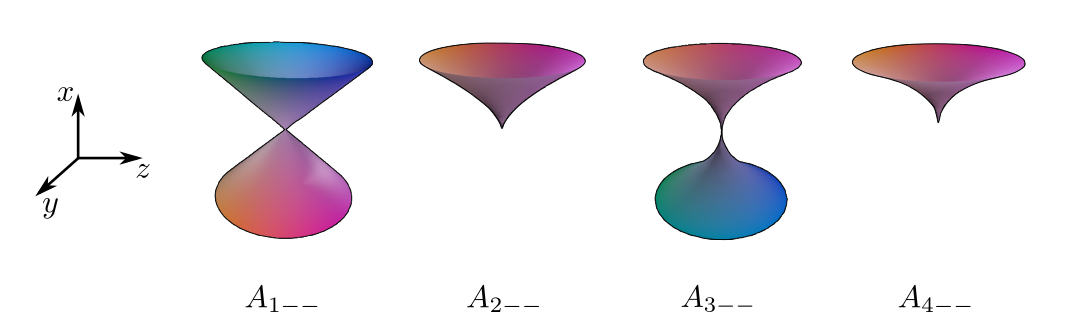
\includegraphics[scale=0.5]{images/img4}}
    \caption[$A_{n--}$ singularities]
    {$A_{n--}$ singularities. \cite{morris2003client}}
    %id obrazku, pomocou ktoreho sa budeme na obrazok odvolavat
    \label{img:4}
\end{figure}


$A_{n+-}$ singularities are topologically equivalent to a cone if $n$ is odd, therefore
they have two branches.
On the contrary with the previous singularities, as $n$ gets bigger, the tip
of the cone gets less sharp and flatter. Branches of these singularities have 
reflection symmetry planes $x=0$ and $y=0$. Therefore we pick the vectors
$(0, 0, 1)$ and $(0, 0, -1)$ as the triangulation vectors.

If $n$ is even, $A_{n+-}$ singularities are topologically equivalent to a plane
with a shape similar to a hyperbolic paraboloid, therefore, they have a single branch.
The first four $A_{n+-}$ singularities can be seen in the Figure~\ref{img:5}.
For this case, we pick the vector $(1, 0, 0)$ as a triangulation vector as
these singularities have reflection symmetry planes $y=0$ and $z=0$.

\begin{figure}
    \centerline{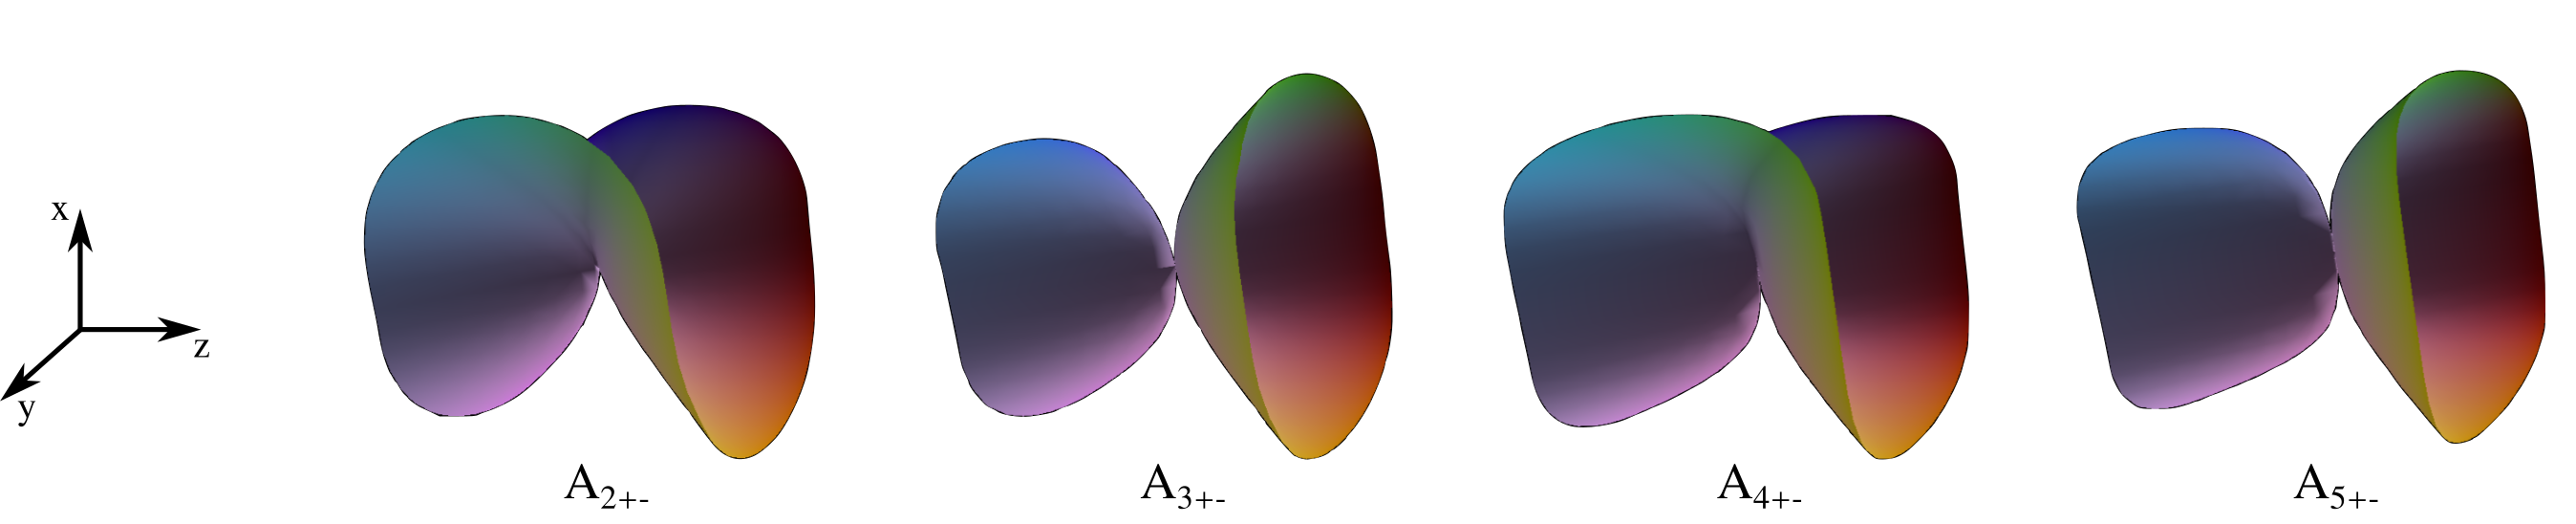
\includegraphics[scale=0.5]{images/img5}}
    \caption[$A_{n+-}$ singularities]
    {$A_{n+-}$ singularities. \cite{morris2003client}}
    %id obrazku, pomocou ktoreho sa budeme na obrazok odvolavat
    \label{img:5}
\end{figure}

\subsubsection*{$D_n$ singularities}

Given by equations $F(x,y,z)=yx^2\pm y^{n-1}\pm z^2$, we consider 8 categories.
For given sign combination and parity of n, the singularities are topologically
equivalent, with sharper(or flatter) features around the singularities for increasing
value of $n$ similar to $A_n$ singularities.

We can therefore say that $D_n$ singularities can be classified into eight categories
locally represented by the following equations:
\begin{itemize}
    \item $D_{4++}$ \hspace{5mm} $yx^2 + y^3 + z^2$
    \item $D_{5++}$ \hspace{5mm} $yx^2 + y^4 + z^2$
    \item $D_{4+-}$ \hspace{5mm} $yx^2 + y^3 - z^2$
    \item $D_{5+-}$ \hspace{5mm} $yx^2 + y^4 - z^2$
    \item $D_{4-+}$ \hspace{5mm} $yx^2 - y^3 + z^2$
    \item $D_{5-+}$ \hspace{5mm} $yx^2 - y^4 + z^2$
    \item $D_{4--}$ \hspace{5mm} $yx^2 - y^3 - z^2$
    \item $D_{5--}$ \hspace{5mm} $yx^2 - y^4 - z^2$.
\end{itemize}

Now we look at some equivalences between these eight categories.
$D_{4++}$ singularity is reflected $D_{4+-}$ singularity.
$D_{5++}$ singularity is reflected $D_{5--}$ singularity.
$D_{5-+}$ singularity is reflected $D_{5+-}$ singularity.
$D_{4-+}$ singularity is reflected $D_{4--}$ singularity.

We therefore only analyze geometry of $D_{n+-}$ singularities and
$D_{n--}$ singularities.

$D_{n+-}$ singularities are topologically equivalent to a plane when $n$ is
even and to a cone when $n$ is odd. Again, as $n$ gets bigger, the features
around singularities get sharper. Symmetry planes of these singularities
are $x=0$ and $z=0$, therefore we pick $(0, 1, 0)$ (and $(0, -1, 0)$ when $n$ is odd)
as triangulation vectors. The first four $D_{n+-}$ singularities can be seen in
the Figure~\ref{img:7}.

\begin{figure}
    \centerline{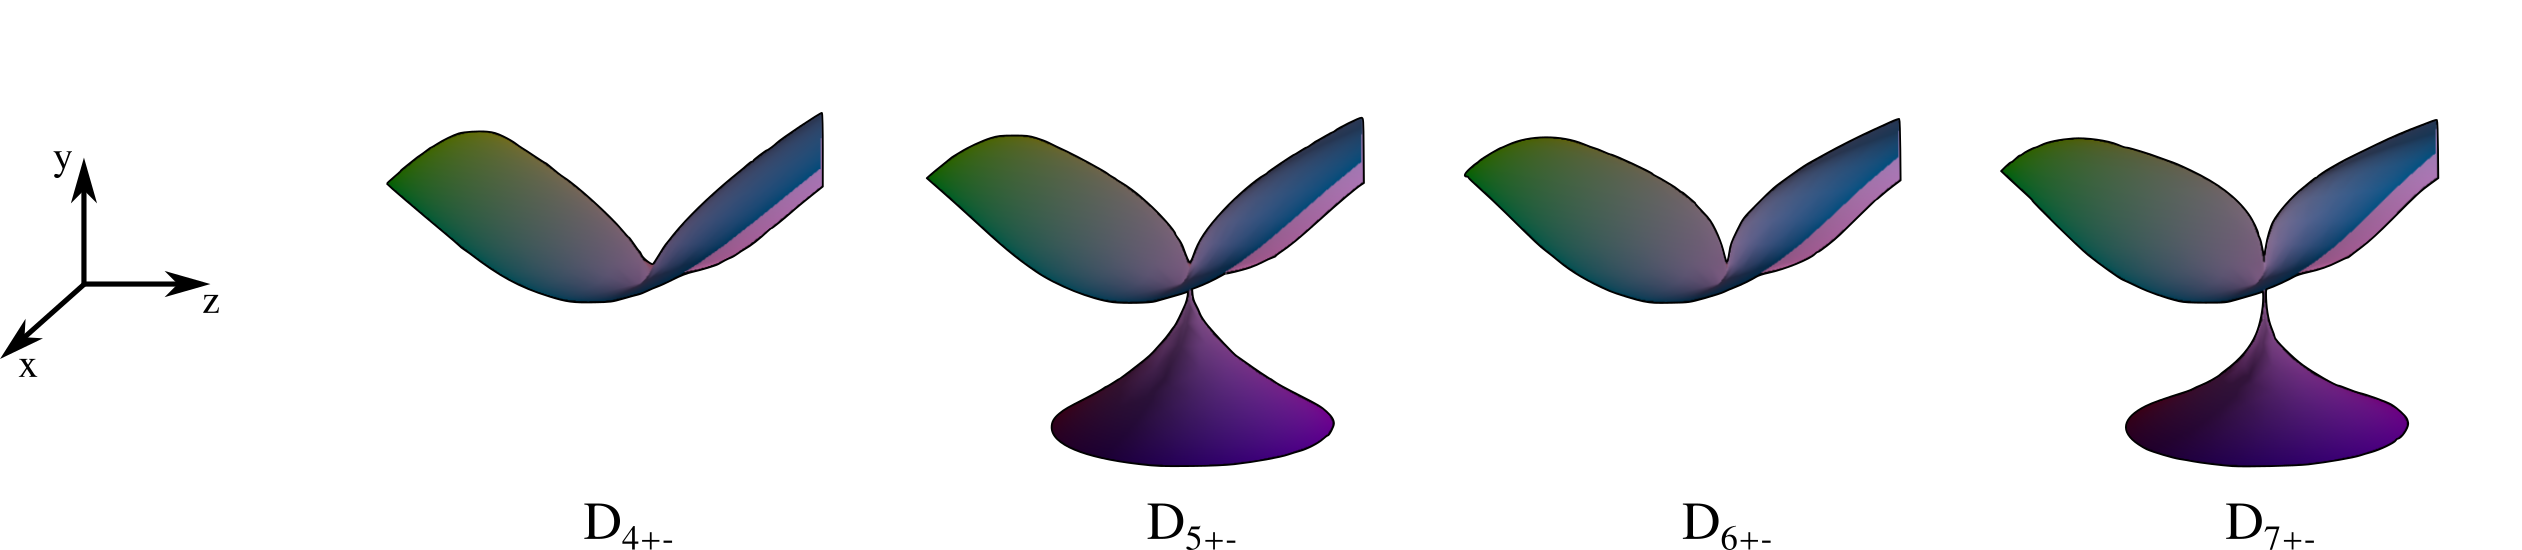
\includegraphics[scale=0.5]{images/img7}}
    \caption[$D_{n+-}$ singularities TODO the coordinates are wrong!!]
    {$D_{n+-}$ singularities. \cite{morris2003client}}
    %id obrazku, pomocou ktoreho sa budeme na obrazok odvolavat
    \label{img:7}
\end{figure}


$D_{n--}$ singularities are topologically equivalent to a cone when $n$ is
odd and to 3 half-cones connected in the singular point when $n$ is even.
First four $D_{n--}$ singularities can be seen in the Figure~\ref{img:8}.

\begin{figure}
    \centerline{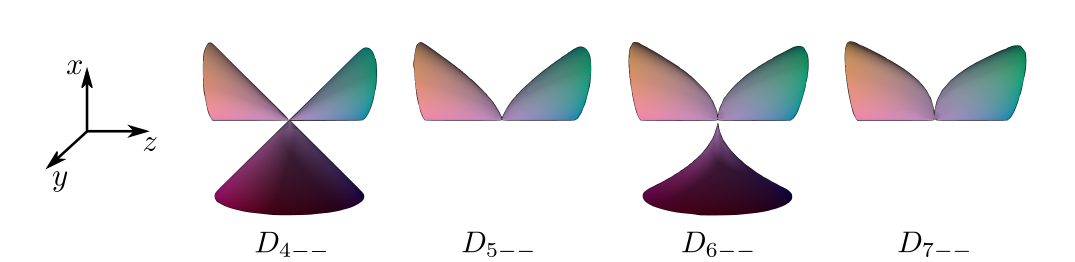
\includegraphics[scale=0.5]{images/img8}}
    \caption[$D_{n--}$ singularities TODO the coordinates are wrong!!]
    {$D_{n--}$ singularities. \cite{morris2003client}}
    %id obrazku, pomocou ktoreho sa budeme na obrazok odvolavat
    \label{img:8}
\end{figure}

The symmetry plane for all branches of these singularities is $z=0$.
the intersection of the surface and plane $z=0$ is displayed on the Figure~\ref{img:6}.

\begin{figure}
    \centerline{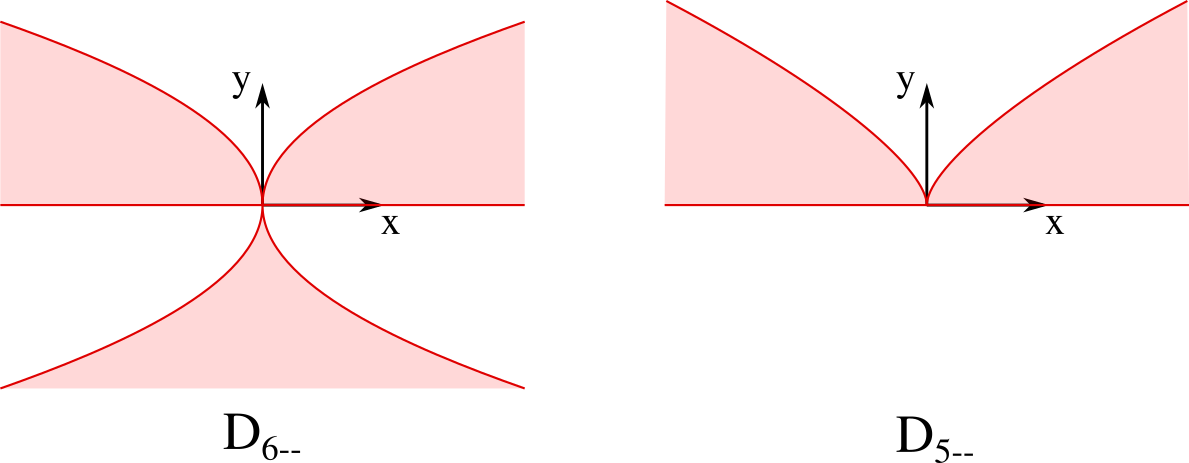
\includegraphics[scale=0.5]{images/img6}}
    \caption[Intersection of $D_{n--}$ singularities with plane $z=0$.]
    {Intersection of $D_{n--}$ singularities with plane $z=0$.}
    %id obrazku, pomocou ktoreho sa budeme na obrazok odvolavat
    \label{img:6}
\end{figure}

For $D_{n--}$ singularity, the intersections of the two branches where
$y \geq 0$ are bounded by curves $y=0$ and $x^2=y^{n-2}$. For given $r$,
we pick the triangulation vectors as $(r, \frac{1}{2}r^{\frac{2}{n-2}}, 0)$
and $(-r, \frac{1}{2}r^{\frac{2}{n-2}}, 0)$. The resulting vectors are
displayed in the Figure~\ref{img:9} by the blue arrow. Parameter $r$ is changed based
on the length of the edge of the triangulation triangle.
displayed on the Figure~\ref{img:9} by blue arrow. Parameter $r$ is changed based
on the length of the edge of the triangulation triangle.

\begin{figure}
    \centerline{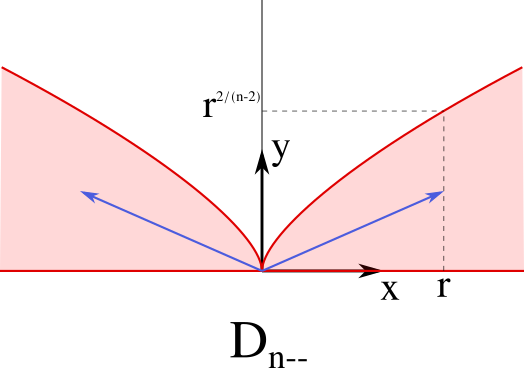
\includegraphics[scale=0.5]{images/img9}}
    \caption[Triangulation vectors for two branches of $D_{n--}$ singularities.]
    {Triangulation vectors for two branches of $D_{n--}$ singularities.}
    %id obrazku, pomocou ktoreho sa budeme na obrazok odvolavat
    \label{img:9}
\end{figure}

The third branch where $y\leq0$ has has another plane of symmetry $x=0$,
therefore triangulation vector for this branch is chosen as $(0, -1, 0)$.

\subsubsection*{$E_6, E_7$ and $E_8$ singularities}

Given by equations $F(x,y,z)=x^3\pm y^4\pm z^2$, $F(x,y,z)=x^3\pm xy^3\pm z^2$
and $F(x,y,z)=x^3\pm y^5\pm z^2$, we can see the following equivalences:
$E_{6++}$ singularity is reflected $E_{6--}$ singularity.
$E_{6+-}$ singularity is reflected $E_{6-+}$ singularity.
$E_{7+-}, E_{7-+}$ and $E_{7--}$ are all reflected $E_{7++}$ singularity.
$E_{8+-}, E_{8-+}$ and $E_{8--}$ are all reflected $E_{8++}$ singularity.

We only analyze geometry of $E_{6++}$, $E_{6+-}$, $E_{7++}$ and $E_{8++}$
singularities. These singularities are displayed in the Figure~\ref{img:12}.


\begin{figure}
    \centerline{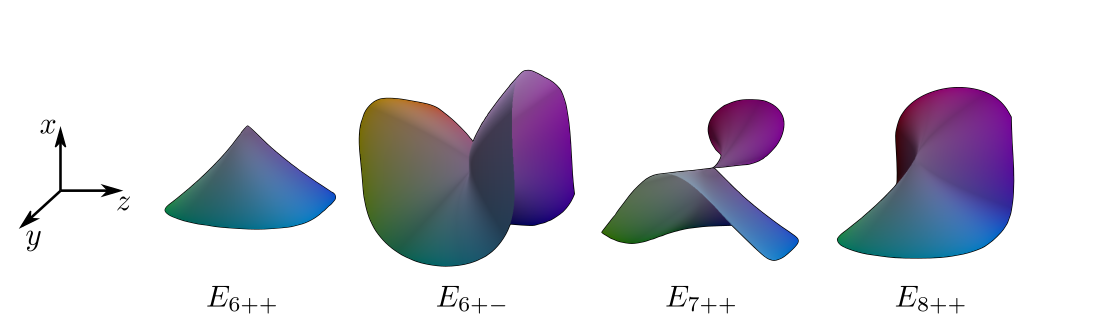
\includegraphics[scale=0.5]{images/img12}}
    \caption[$E_n$ singularities.]
    {$E_n$ singularities \cite{morris2003client}.}
    %id obrazku, pomocou ktoreho sa budeme na obrazok odvolavat
    \label{img:12}
\end{figure}
Both $E_{6++}$ and $E_{6+-}$ are topologically equivalent to a plane, thus
they each have only one branch. The planes of symmetry of both of these 
branches are $y=0$ and $z=0$, therefore we pick $(-1, 0, 0)$ as the
triangulation vector.

$E_{7++}$ singularity is topologically equivalent to a cone, therefore, it has
two branches. The plane of symmetry of this singularity is $z=0$.

$E_{8++}$ singularity is also topologically equivalent to a plane, therefore,
it has only one branch. This branch has only one plane of symmetry $z=0$.

We again look at the intersection of the surfaces with the plane of 
symmetry, this is displayed in the Figure~\ref{img:10}.

\begin{figure}
    \centerline{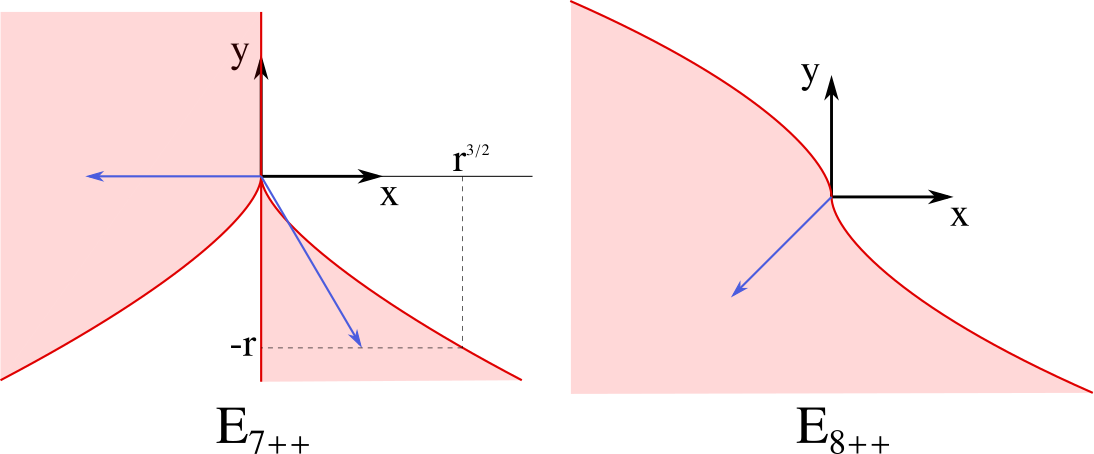
\includegraphics[scale=0.5]{images/img10}}
    \caption[Intersection of $E_{7++}$ and $E_{8++}$ singularities with 
    plane $z=0$.]
    {Intersection of $E_{7++}$ and $E_{8++}$ singularities with 
    plane $z=0$.}
    %id obrazku, pomocou ktoreho sa budeme na obrazok odvolavat
    \label{img:10}
\end{figure}

For $E_{7++}$ singularity, we pick $(-1, 0, 0)$ and 
$(\frac{1}{2}r^{\frac{3}{2}}, -r, 0)$ as triangulation vectors.
For $E_{8++}$ singularity, we pick $(-1, -1, 0)$ as a triangulation vector.
These vectors are displayed as blue arrows in the Figure~\ref{img:10}.

\subsection{Analytical calculation of local triangulation of some ADE singularities}
For given edge size $e$, we calculate the local triangulation of ADE
singularities, such that edges on the border of the local triangulation
have length $e$.
\subsubsection*{$A_{n--}$ singularities}
\label{An--singularities}
For $A_{n--}$ singularities, we create a disc of six isosceles triangles
with a vertex in the singular point. The bases of these triangles create regular
hexagon in the plane $P$ parallel to the plane $x=0$, as showed on the Figure
\ref{img:11}.
\begin{figure}
    \centerline{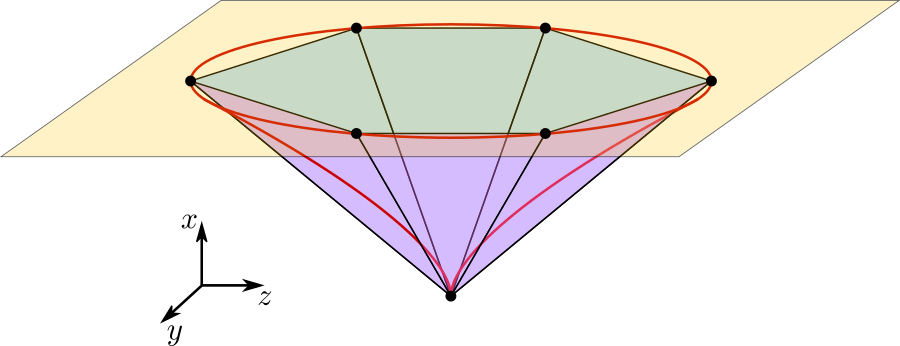
\includegraphics[scale=0.5]{images/img11}}
    \caption[Triangulation of $A_{n--}$ singularity.]
    {Triangulation of $A_{n--}$ singularity.}
    %id obrazku, pomocou ktoreho sa budeme na obrazok odvolavat
    \label{img:11}
\end{figure}
Given by equation $x^{n+1}-y^2-z^2=0$, we find the distance of the 
plane $P$ from the plane $x=0$ for the given length $e$ of the sides of
the hexagon.

Let $e$ be the length of the side of the hexagon, then the circumscribed
circle has radius $e$. This circle is identical with the intersection of
the surface and the plane $x=h$. The equation of the intersecting circle
is $y^2+z^2=h^{n+1}$ therefore, the radius can be also expressed as 
$r=h^{\frac{n+1}{2}}$, which emerges $h=e^{\frac{2}{n+1}}$. Knowing the
distance of the plane, one can easily calculate the length of the arms of
the triangles using the Pythagorean theorem: 
$$a^2=h^2+e^2 \implies a = \sqrt{e^{\frac{4}{n+1}} + e^2}$$

\textbf{Layers for $A_{n--}$ singularities:}
The resulting mesh with uniform triangles for $A_{5--}$ singularity is displayed
on the Figure~\ref{img:A5-uniform}.  

\begin{figure}
    \centerline{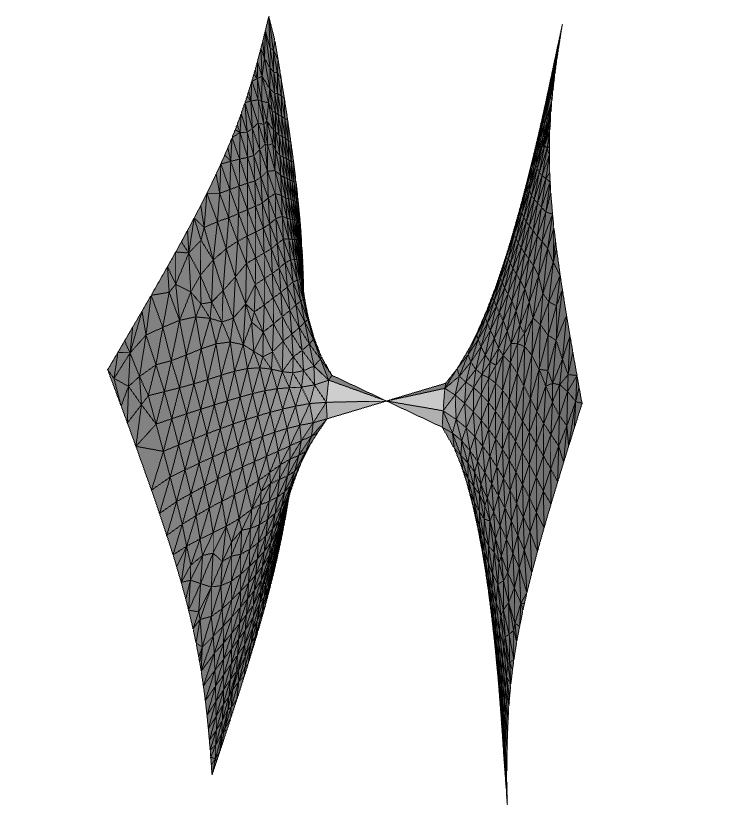
\includegraphics[scale=0.25]{images/A5-uniform}}
    \caption[Resulting uniform triangulation of the $A_{5--}$ singularity]
    {Resulting uniform triangulation of the $A_{5--}$ singularity.}
    %id obrazku, pomocou ktoreho sa budeme na obrazok odvolavat
    \label{img:A5-uniform}
\end{figure}

As one may see, the approximation around the singular
point is less accurate than for the rest of the surface.
For this problem, we introduce layers -- the surroundings of singularities are
triangulated in multiple layers of triangles, and only after that, the algorithm for
regular parts is used.

Given the edge length $e$ and number of layers, we calculate the height $h_e$ 
at which the bases of the triangles
have the length $e$. We divide the height by the number of layers to obtain the
layer height $h_l$. Now, $i$--th layer of points is obtained using the height
$h = i\cdot h_l$. To connect these points into triangles, every second
layer is rotated by $\frac{\pi}{6}$. The resulting 3 layers of triangles
for the $A_{1--}$ singularity as viewed from the point $(1, 0, 0)$ is displayed on
the Figure~\ref{img:52}. 

\begin{figure}
    \centerline{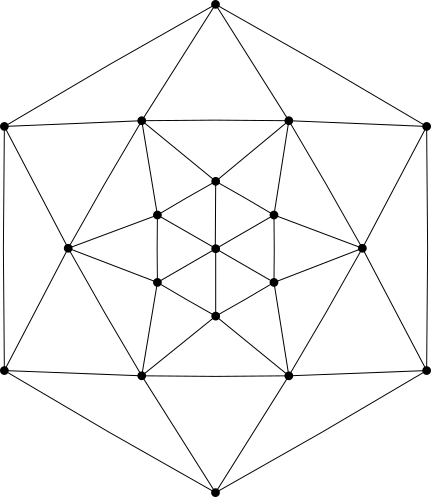
\includegraphics[scale=0.5]{images/img52}}
    \caption[Three layers of triangles for the $A_{1--}$ singularity]
    {Three layers of triangles for the $A_{1--}$ singularity.}
    %id obrazku, pomocou ktoreho sa budeme na obrazok odvolavat
    \label{img:52}
\end{figure}

The local mesh with one layer, four layers and eight layers (from left to right) 
for $A_{5--}$ singularity is displayed
on the Figure~\ref{img:53}. 
\begin{figure}
    \centerline{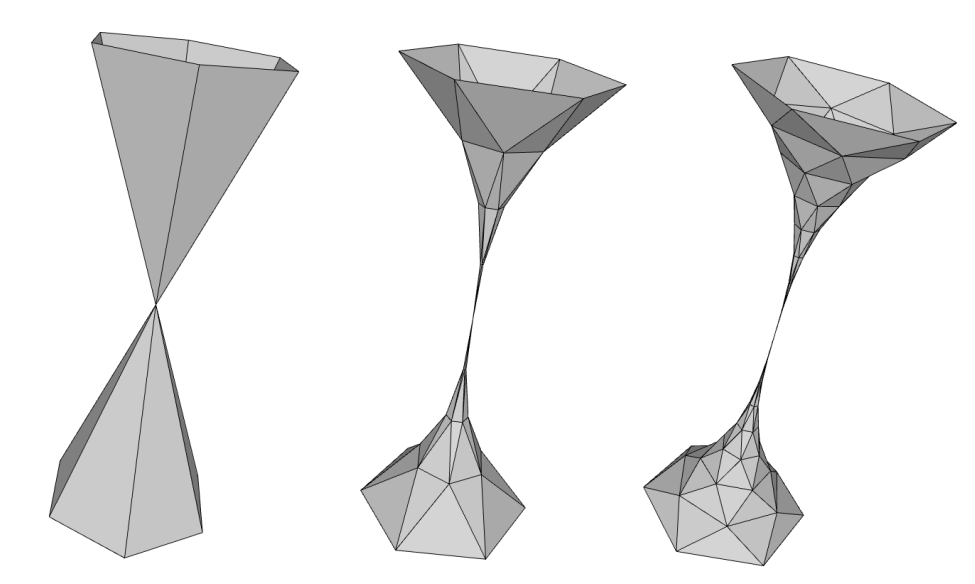
\includegraphics[scale=0.4]{images/img53}}
    \caption[Local mesh with layers for the $A_{5--}$ singularity]
    {Local mesh with one layer, four layers and eight layers (from left to right) 
    for the $A_{5--}$ singularity.}
    %id obrazku, pomocou ktoreho sa budeme na obrazok odvolavat
    \label{img:53}
\end{figure}

The resulting mesh with four layers is displayed on the
Figure~\ref{A5-uniform-layers}.
\begin{figure}
    \centerline{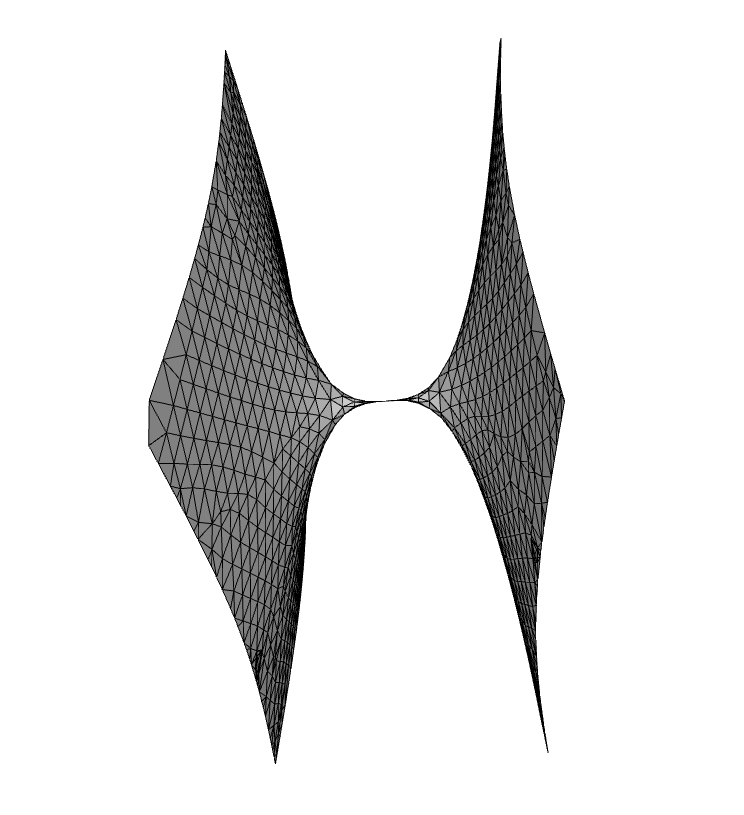
\includegraphics[scale=0.25]{images/A5-uniform-layers}}
    \caption[Resulting mesh for the $A_{5--}$ singularity]
    {Resulting mesh for the $A_{5--}$ singularity - four layers.}
    %id obrazku, pomocou ktoreho sa budeme na obrazok odvolavat
    \label{img:A5-uniform-layers}
\end{figure}

\subsubsection*{$D_n$ singularities}
Some $D_n$ singularities have branches with elliptical intersection with 
a plane parallel to the plane $y=0$. As ellipses have two axes of symmetry,
we create eight triangles with an apex in the singular point for these branches.
The other points of the triangles lie on the ellipse, and they have the same base length.

Let us have an ellipse $E$ with semi-major axis $a$, semi-minor axis $b$ 
and the center in the point $(0, 0)$.

$$E: \frac{x^2}{a^2} + \frac{y^2}{b^2} = 1$$
\begin{figure}
    \centerline{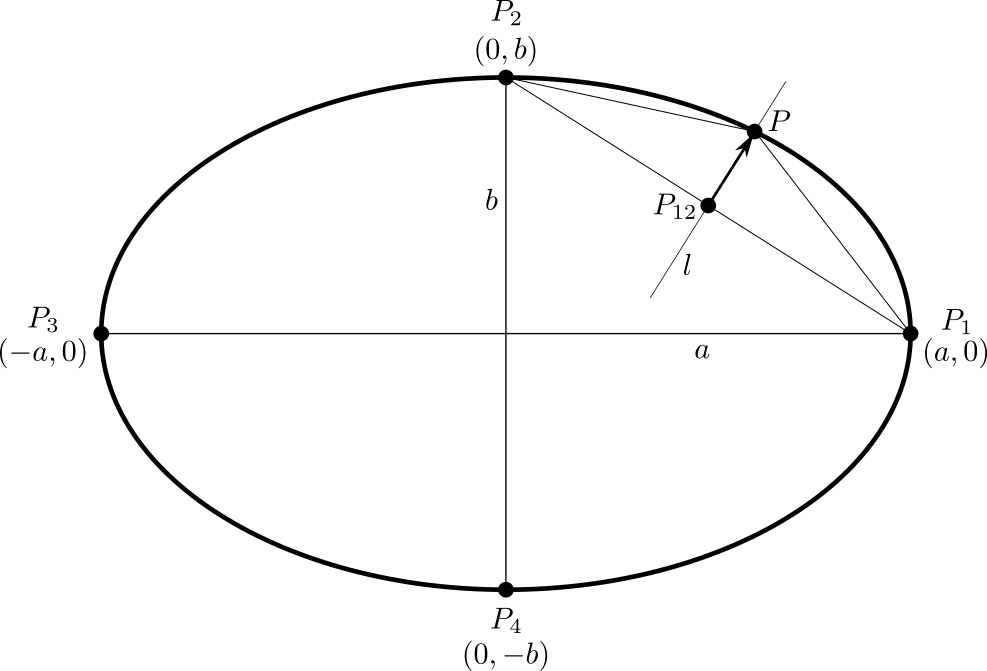
\includegraphics[scale=0.5]{images/img13}}
    \caption[Equidistant points on ellipse.]
    {Equidistant points on the ellipse.}
    %id obrazku, pomocou ktoreho sa budeme na obrazok odvolavat
    \label{img:13}
\end{figure}
As displayed in the Figure~\ref{img:13}, we pick the leftmost, the rightmost, the top
and the bottom points. As shown on the figure~\ref{img:13}, the coordinates of these 
points are $P_1 = (a, 0)$, $P_2 = (0, b)$, $P_3=(-a, 0)$, $P_4 = (0, -b)$.
Then we can calculate the point $P$ on the ellipse equidistant
from points $P_1$ and $P_2$. We calculate this point by taking the point $P_{12}$ 
in the middle of a line segment $P_1P_2$. 

$$P_{12} = \frac{1}{2}(a, b)$$

Then, the point $P$ is lying on the
intersection of the ellipse and a line $l$ passing through the point $P_{12}$, perpendicular to the
line segment $P_1P_2$.

$$l: \frac{1}{2}(a,b) + \frac{t}{2}(b,a), \hspace{3mm} t \in \R$$

Given the ellipse with semi-major axis $a$, 
semi-minor axis $b$ and the center in the point $(0, 0)$, the point $P$ can be 
calculated as follows

$$P \in l \cap E \implies 
\frac{(a+tb)^2}{4a^2} + \frac{(b+ta)^2}{4b^2} = 1$$
$$t=\frac{ab(\sqrt{3a^4+2a^2b^2+3b^4}-a^2-b^2)}{a^4+b^4},$$
therefore 
$$P=\frac{1}{2}(a,b) + \frac{ab(\sqrt{3a^4+2a^2b^2+3b^4}-a^2-b^2)}{2(a^4+b^4)}(b,a).$$

Given edge length $e$, we are not able to calculate the height in which the distance
between points $P1$ and $P$ is $e$. The visualization showing this is in the Figure~\ref{img:17}.

\begin{figure}
    \centerline{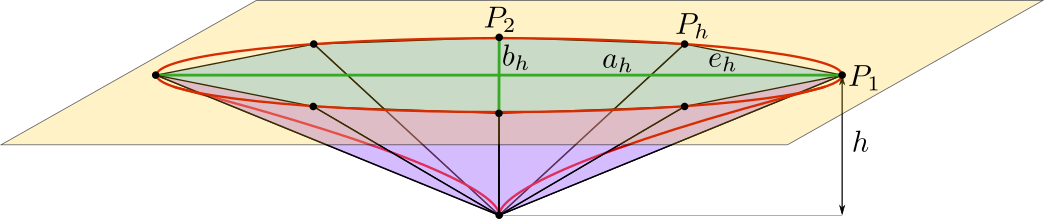
\includegraphics[scale=0.5]{images/img17}}
    \caption[Calculating the point $P_h$]
    {Calculating the point $P_h$ -- point on the ellipse equidistant from $P_1$ and $P_2$.}
    %id obrazku, pomocou ktoreho sa budeme na obrazok odvolavat
    \label{img:17}
\end{figure}

We use binary search to find such height.
Given the height and the singularity class, we can calculate the semi-major axis
and semi-minor axis as 

$$D_{n+-} \hspace{3mm} :\hspace{3mm}  -hx^2+h^{n-1}-z^2 = 0 \hspace{5mm} h>0$$
$$x^2 + \frac{z^2}{h} = h^{n-2}$$
$$\frac{x^2}{h^{n-2}} + \frac{z^2}{h^{n-1}} = 1 \implies a_h=max(h^\frac{n-2}{2}, h^\frac{n-1}{2}) \land b_h=min(h^\frac{n-2}{2}, h^\frac{n-1}{2}).$$

As we can see, we get the same ellipse for $D_{n--}$ singularities:

$$D_{n--} \hspace{3mm} :\hspace{3mm}  -hx^2-h^{n-1}-z^2 = 0 \hspace{5mm} h>0$$
$$2|n \land x^2 + \frac{z^2}{h} = -h^{n-2} \implies x^2 + \frac{z^2}{h} = h^{n-2}.$$
Then 
$$P_h=\frac{1}{2}(h^\frac{n-2}{2},h^\frac{n-1}{2}) + \frac{h^\frac{2n-3}{2}(\sqrt{3h^{2n-4}+2h^{2n-3}+3h^{2n-2}}-h^{n-2}-h^{n-1})}{2(h^{2n-4}+h^{2n-2})}(h^\frac{n-1}{2},h^\frac{n-2}{2})$$
$$P_h=\frac{1}{2}(h^\frac{n-2}{2},h^\frac{n-1}{2}) + \frac{h^\frac{1}{2}(\sqrt{3+2h+3h^2}-1-h)}{2(1+h^2)}(h^\frac{n-1}{2},h^\frac{n-2}{2})$$
and we can calculate $e_h=||P_h-P_1||$.

As $e \leq a_h$, we can start the binary search on the interval
$\langle 0, a^\frac{2}{n-2}\rangle$ or $\langle 0, a^\frac{2}{n-1}\rangle$
and finish when the required precision is reached.

\textbf{Proof that $e_h$ is monotone in $h$:} Let us consider a general ellipse
with the semi-major axis $a$, semi-minor axis $b$ and center in the point $(0, 0)$. 
Let us denote the points as follows: $A=(a, 0)$, $B=(0, b)$, $M=(\frac{a}{2}, \frac{b}{2})$ 
and $C$ - point in the first quadrant of the ellipse equidistant from $A$ and $B$, the points
are displayed on the Figure~\ref{img:40}.

\begin{figure}
    \centerline{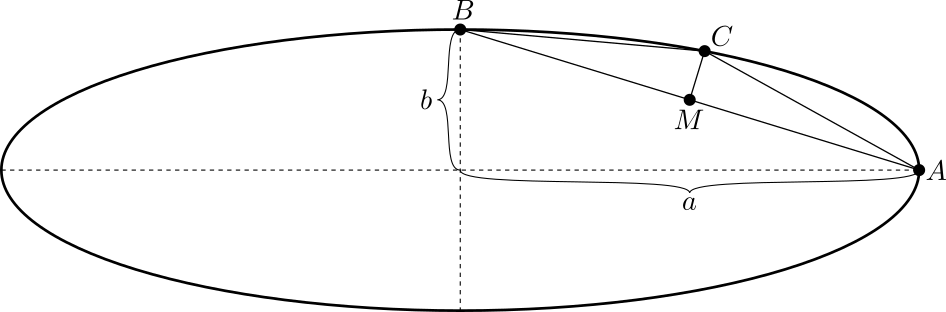
\includegraphics[scale=0.5]{images/img40}}
    \caption[Notation used in the proof]
    {Notation used in the proof that $e_h$ is monotone in $h$.}
    %id obrazku, pomocou ktoreho sa budeme na obrazok odvolavat
    \label{img:40}
\end{figure}

As we calculated, it holds that
$$C = M + \frac{t}{2} \cdot (b, a) \hspace{5mm} \textrm{for} \hspace{5mm} t=\frac{ab(\sqrt{3a^4+2a^2b^2+3b^4}-a^2-b^2)}{a^4+b^4}.$$

As length of the vector $(b,a)$ is $\sqrt{a^2+b^2}$, the distance 
$|MC|$ is $\frac{t}{2} \cdot \sqrt{a^2+b^2}$.

After substituing for $t$, one gets 
$$|MC|=\sqrt{a^2+b^2}\cdot\frac{ab(\sqrt{3a^4+2a^2b^2+3b^4}-a^2-b^2)}{2(a^4+b^4)},$$
the derivative $\frac{\partial|MC|}{\partial a}$ is positive for all $b>0$ and
$\frac{\partial|MC|}{\partial b}$ is positive for all $a>0$.

This means that $|MC|$ is increasing in both $a$ and $b$. As the distance $|MA|=|MB|$ is 
also increasing in $a$ and $b$, it follows from Pythagorean theorem, that $|AC|=|BC|$
is increasing in $a$ and $b$.

When the height $h$ increases, both the semi-major and semi-minor axis of the ellipse increase,
thus $e_h$ is increasing in $h$.

\subsection{Numerical calculation of local triangulation of ADE singularities}

The exact analytical calculations become more
complicated for other types of ADE singularities. In this section, we present an approach for triangulation of all types
of ADE singularities using iterative numerical algorithms based on the binary 
search.

We begin by dividing ADE singularities into two categories.
\begin{enumerate}
    \item Category singularities -- displayed on the Figure~\ref{img:42}:
    \begin{itemize}
        \item $A_{n--}$,
        \item $A_{n+-}$,
        \item $D_{n+-}$, where $n=2k$,
        \item $E_{6++}$, 
        \item $E_{6+-}$,
        \item $E_{8++}$.
    \end{itemize}
    \begin{figure}
        \centerline{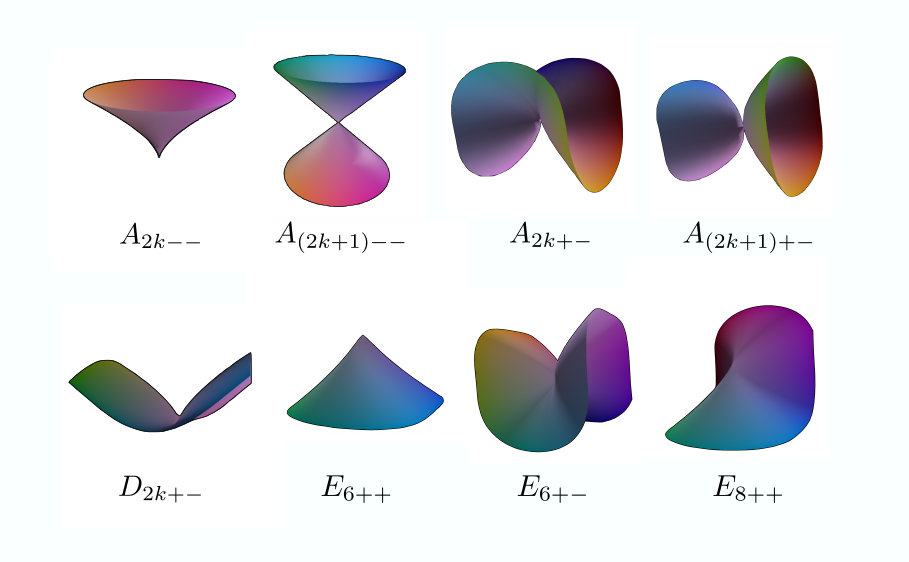
\includegraphics[scale=0.5]{images/img42}}
        \caption[1. Category singularities]
        {1. Category singularities \cite{morris2003client}.}
        %id obrazku, pomocou ktoreho sa budeme na obrazok odvolavat
        \label{img:42}
    \end{figure}
    \item Category singularities -- displayed on the Figure~\ref{img:43}:
    \begin{itemize}
        \item $D_{n+-}$, where $n=2k+1$,
        \item $D_{n--}$,,
        \item $E_{7++}$.
    \end{itemize}
    \begin{figure}
        \centerline{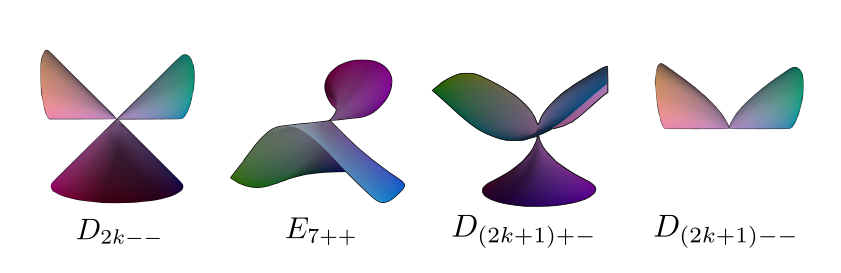
\includegraphics[scale=0.5]{images/img43}}
        \caption[2. Category singularities]
        {2. Category singularities \cite{morris2003client}.}
        %id obrazku, pomocou ktoreho sa budeme na obrazok odvolavat
        \label{img:43}
    \end{figure}
\end{enumerate}

\subsubsection*{Triangulation of 1. category singularities}
For all of the singularities, we have defined the triangulation vector,
let us denote the normalized triangulation vector of the singularity 
as $\vec{t}$, resp. $\vec{t}_1, .., \vec{t}_i$ if the 
singularity has $i$ triangulation vectors.
Let us assume that the singular point is located in the point $O = (0, 0, 0).$
For the singularities from 1. category, 
topologically equivalent to a plane, given by the implicit
equation $F(x, y, z) = 0$ it holds, that $F(O+\vec{t}) \cdot F(O-\vec{t})<0$.
For the singularities from the 2. category, topologically equivalent to a cone,
it holds, that $F(O+\vec{t}_j) \cdot F(O+\vec{t}_j^\bot) <0$ for $j = 0, 1$.
This means that in both cases, we can perform a binary search to find a point on 
the surface.
Given the required length $l$ -- the length of the leg of the isosceles triangle 
created around the singularity, we perform a binary search to find
an angle, for which the endpoint of the rotated vector $l \cdot \vec{t}$ lies on 
the surface with given precision as displayed in the Figure~\ref{img:41}.

\begin{figure}
    \centerline{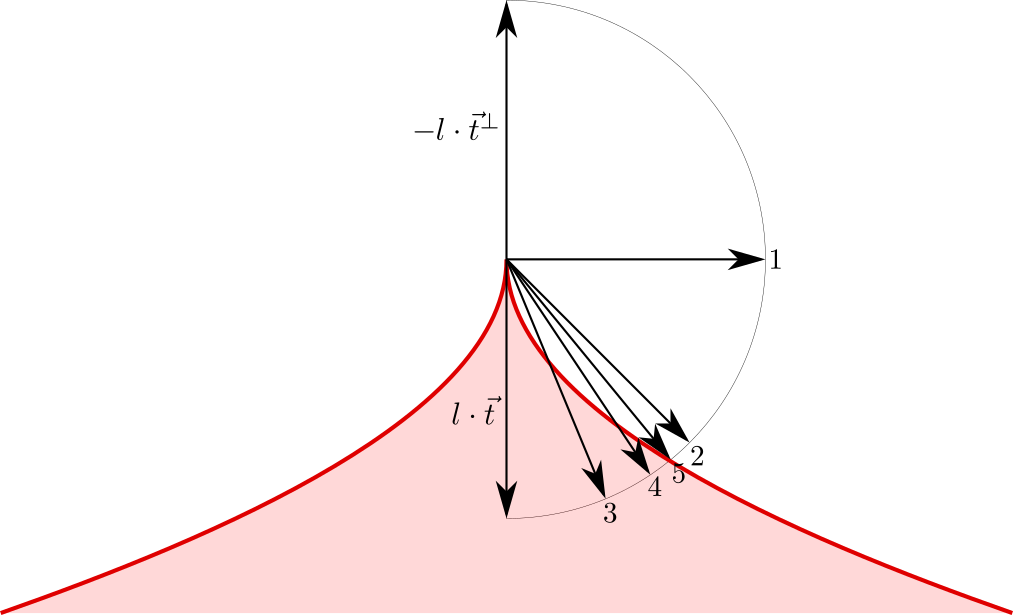
\includegraphics[scale=0.5]{images/img41}}
    \caption[Binary search for the point on the surface]
    {Binary search for the point on the surface.}
    %id obrazku, pomocou ktoreho sa budeme na obrazok odvolavat
    \label{img:41}
\end{figure}

The binary search for singularities topologically equivalent to a cone is displayed
on the Figure~\ref{img:45}.

\begin{figure}
    \centerline{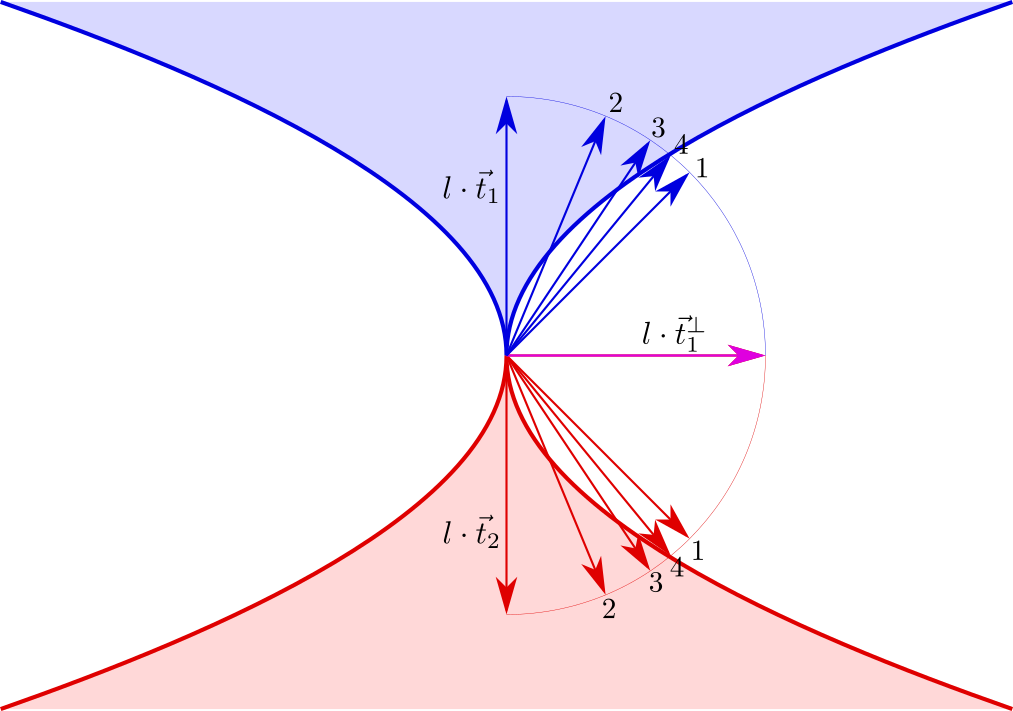
\includegraphics[scale=0.5]{images/img45}}
    \caption[Double binary search for the point on the surface]
    {Double binary search for the point on the surface.}
    %id obrazku, pomocou ktoreho sa budeme na obrazok odvolavat
    \label{img:45}
\end{figure}

The binary search is performed in the half-planes passing through the point
$O$ and with the vector $\vec{t}$ lying in the half-planes.
Using this approach, we create $k$ points on the surface, while each time
rotating the half-plane in which the binary search is performed by $\frac{2\pi}{k}$
about the axis given by $\vec{t}$ as displayed on the Figure~\ref{img:rotating-planes}.

\begin{figure}
    \centerline{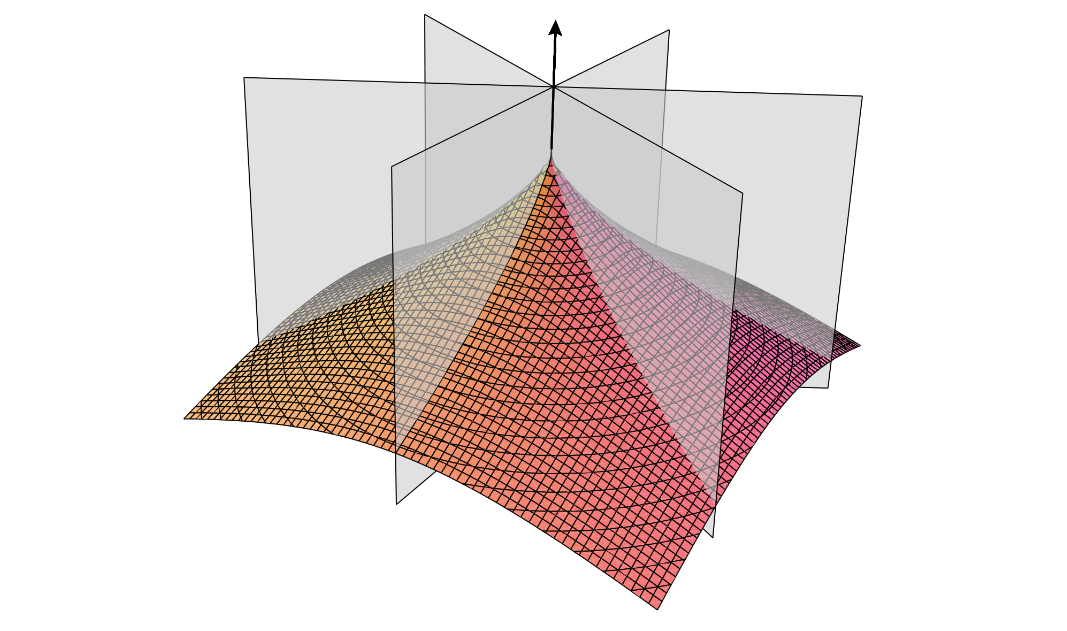
\includegraphics[scale=0.3]{images/rotating-planes}}
    \caption[Rotating the plane about the vector]
    {Rotating the plane about the vector $\vec{t}$ \cite{calcplot3d}.}
    %id obrazku, pomocou ktoreho sa budeme na obrazok odvolavat
    \label{img:rotating-planes}
\end{figure}

For $A_{n--}$ singularities, we create six
triangles near the singular point. We only need to perform the binary search once,
other points are obtained by rotating the point on the surface about the vector 
$\vec{t}$ by $\frac{2 \pi}{6}$.

For $A_{n--}$ singularities with two branches, the same approach is used,
we perform the binary search only once and use rotation and
reflection to create the remaining points on the surface.

In the case of other singularities, we create different numbers of triangles:
\begin{itemize}
    \item $A_{2k+-}$ -- 8 triangles,
    \item $A_{(2k+1)+-}$ -- 6 triangles for each branch,
    \item $D_{2k+-}$ -- 8 triangles for the branch given by the 
    triangulation vector $(0,1,0)$ and 4 triangles for the branch
    given by the triangulation vector $(0,-1,0)$,
    \item $D_{(2k+1)+-}$ -- 8 triangles,
    \item $D_{2k--}$ -- 4 triangles for each branch,
    \item $E_{6++}$ -- 6 triangles,
    \item $E_{6+-}$ -- 8 triangles,
    \item $E_{7++}$ -- 6 triangles for the branch, given by the
    triangulation vector $(-1, 0, 0)$ and 4 triangles for the other
    branch,
    \item $E_{8++}$ -- 6 triangles.
\end{itemize}

As some singularities have symmetries, we can use these symmetries
to perform the binary search fewer times and find the remaining points
as the mirror symmetries of the points found by binary search.

\subsubsection*{Triangulation of 2. category singularities}
We create a more general, slower solution for the singularities in the 2. category.
Again, we find the points on the surface lying in the rotated half-planes
as displayed on the Figure~\ref{img:rotating-planes}.
We do not have the general rule for the start 
and end angle to begin the binary search for these singularities. We have the triangulation vector,
whose endpoint lies inside the space volume bounded by the respective branch.
We consider this triangulation vector a start vector to start the binary 
search. We find the end vector by rotating the triangulation vector $\vec{t}$ 
around the vector $\vec{p}$ -- vector perpendicular to $\vec{t}$, by small increments, 
until the endpoint of the rotated vector is outside of the space volume bounded by the branch,
let us denote this vector $\vec{r}$.
To find the point of the surface, we perform an angular binary search between $\vec{t}$
and $\vec{r}$. We proceed to find other points by rotating $\vec{p}$
around $\vec{t}$ by $\frac{2\pi}{k}$.
By using the small increments, we ensure that the rotated vector does not end up in
the space volume bounded by another branch, but it slows down the process of creating
the local mesh.
For the illustration, in the Figure~\ref{img:54} on the left, one can see the iterative
process to find the vector $\vec{r}$ by rotating $\vec{t}$ around $\vec{p}$.
On the right, one can see the rotation of $\vec{p}$ around $\vec{t}$ by 
$\frac{2\pi}{k}$ to find the remainding points on the surface.

\begin{figure}
    \centerline{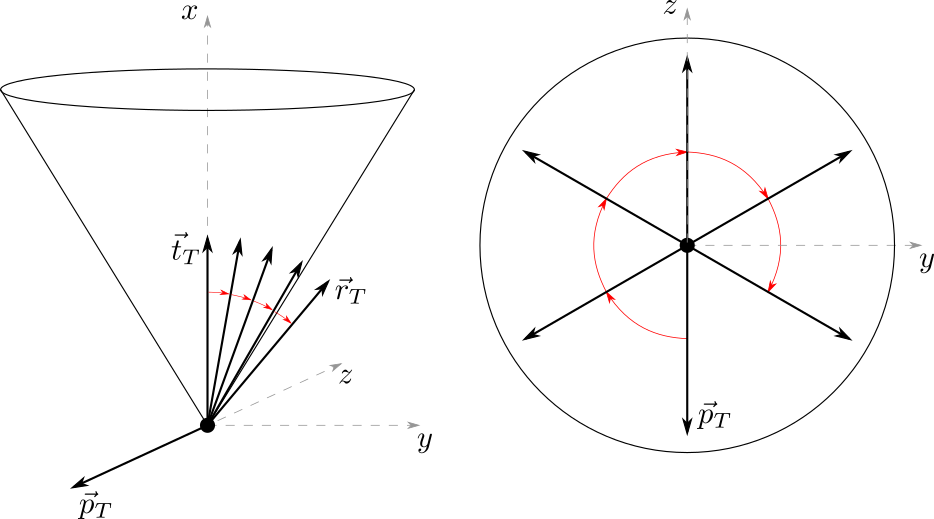
\includegraphics[scale=0.5]{images/img54}}
    \caption[Triangulation of 2. category singularities]
    {Iterative process of finding the vector $\vec{r}$ 
    by rotating $\vec{t}$ around $\vec{p}$ (left).
    Rotating the vector $\vec{p}$ around $\vec{t}$ by 
    $\frac{2\pi}{k}$ (right).}
    %id obrazku, pomocou ktoreho sa budeme na obrazok odvolavat
    \label{img:54}
\end{figure}

For the singularities with rotation
symmetry, we only need to perform the binary search once and create the remaining 
points using rotation symmetry.
In the case of other singularities with different symmetries, we again make use of the
potential planes of symmetry to find the points on the surface.

\subsubsection*{Layers for ADE singularities}
We have already introduced the concept of creating multiple layers of triangles around
$A_{n--}$ singularities. In this section, we explain the extension of this concept
to remaining ADE singularities. We create $l$ layers of
points for each branch for a given singularity. In contrast with $A_{n--}$ singularities, we do not 
rotate every second layer by $\frac{\pi}{k}$. The reason is that the midpoints of
the edges connecting a particular layer of points do not lie on the surface. This results
in a poor approximation of the curves lying in the intersection of the surface 
and coordinate planes. Sometimes, it even results in incorrect local mesh with 
overlapping triangles.

In the Figure~\ref{img:56} on the left, one may see the insufficient approximation
of $D_{4+-}$ singularity with
four layers of triangles and rotation by $\frac{\pi}{k}$. On the right, one
may see the local mesh of the same singularity with four layers of triangles
without rotation by the angle $\frac{\pi}{k}$.

\begin{figure}
    \centerline{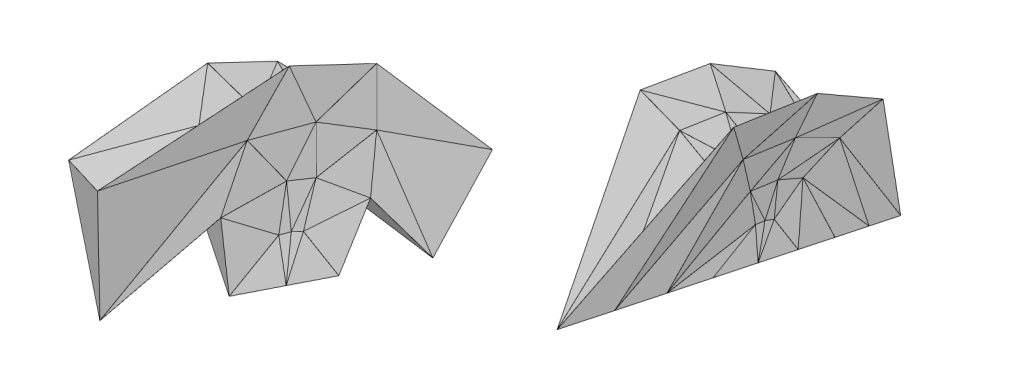
\includegraphics[scale=0.4]{images/img56}}
    \caption[Insufficient and sufficient local approximation]
    {Insufficient (left) and sufficient (right) local approximation of $D_{4+-}$ singularity.}
    %id obrazku, pomocou ktoreho sa budeme na obrazok odvolavat
    \label{img:56}
\end{figure}

On the Figure~\ref{img:55} on the left, one may see the incorrect local mesh
of $A_{2+-}$ singularity with
two layers of triangles and rotation by $\frac{\pi}{k}$. On the right, one
may see the local mesh of the same singularity with two layers of triangles
without rotation by the angle $\frac{\pi}{k}$.

\begin{figure}
    \centerline{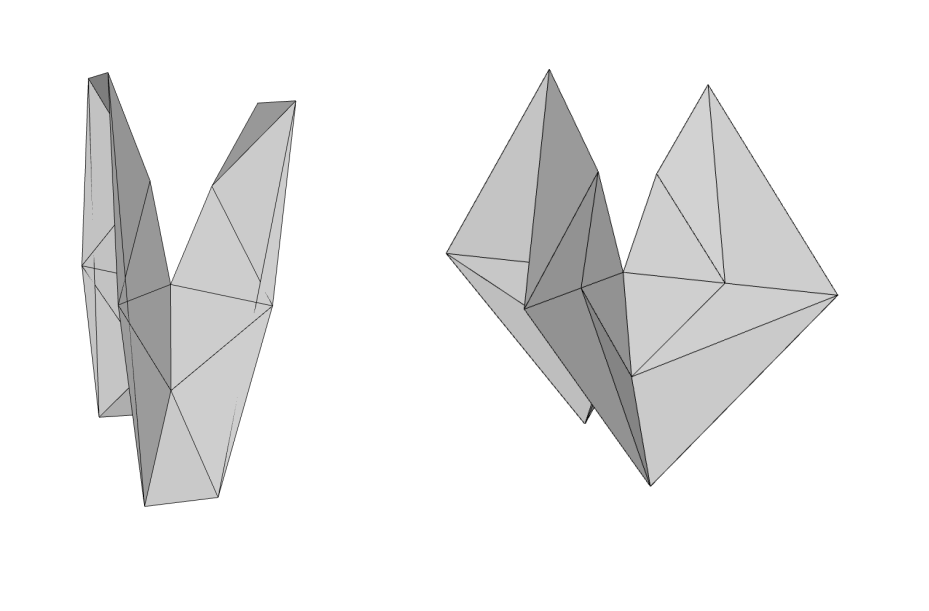
\includegraphics[scale=0.4]{images/img55}}
    \caption[Incorrect and correct local mesh]
    {Incorrect (left) and correct (right) local mesh for $A_{2+-}$ singularity.}
    %id obrazku, pomocou ktoreho sa budeme na obrazok odvolavat
    \label{img:55}
\end{figure}


\subsubsection*{Optimization of the quality of the local mesh for some singularities}
For some of the singularities, it is not convenient to look for the points on
the surface in the planes rotated by identical angles as seen in the Figure
\ref{img:rotating-planes}. An example of such singularities are $D_{n+-}$
singularities. The local mesh created with eight triangles using the described 
approach is displayed in the Figure~\ref{img:D4-before}. One may see that the
outer edges of the triangles have a significant length difference.

\begin{figure}
    \centerline{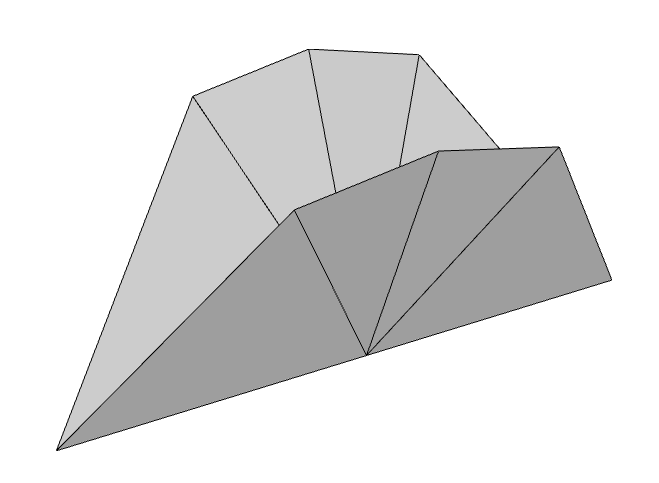
\includegraphics[scale=0.25]{images/D4-before}}
    \caption[Uneven triangles in the local mesh around $D_{4+-}$ singularity]
    {Uneven triangles in the local mesh around $D_{4+-}$ singularity.}
    %id obrazku, pomocou ktoreho sa budeme na obrazok odvolavat
    \label{img:D4-before}
\end{figure}

The problem is significant in the singularities with eight triangles near
the singular point.
Our solution is to use binary search to find the angle where the triangles are
close to isosceles triangles. The points found in rotated half-spaces given by 
the angles $0, \frac{\pi}{2}, \pi$ and $\frac{3\pi}{4}$ are unchanged.
The points between these points are iteratively changed until the
triangles are isosceles with the required precision. Starting on the interval 
of angles $(0, \frac{\pi}{2})$, in each step, 
the new angle is calculated as an angle in the middle 
between the two angles. The new point is then calculated using the binary 
search to find a point on the surface as displayed in the Figure~\ref{img:41}.

As all singularities using this optimization are symmetrical by two coordinate
planes, we only need to perform this binary search once for each layer of 
points and use mirror symmetry to obtain the remaining points.

The result of the binary 
search of an angle for the $D_{4+-}$ singularity is displayed 
on the Figure~\ref{img:D4-after}. The triangles around the singularity
are closer to isosceles triangles in comparison to the Figure 
\ref{img:D4-before}.

\begin{figure}
    \centerline{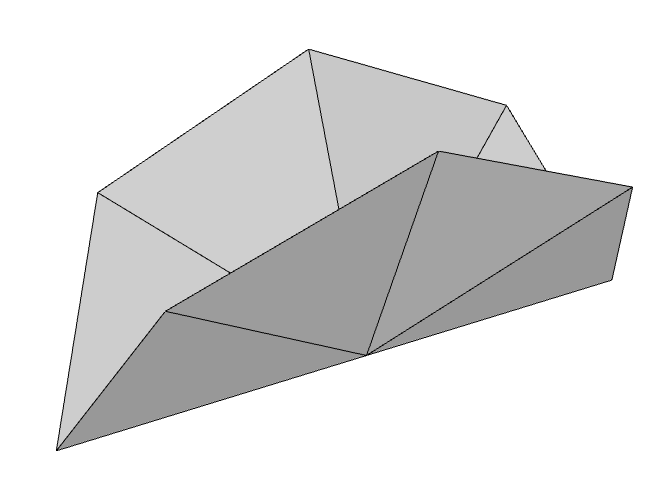
\includegraphics[scale=0.25]{images/D4-after}}
    \caption[Optimized local mesh around $D_{4+-}$ singularity]
    {Optimized local mesh around $D_{4+-}$ singularity.}
    %id obrazku, pomocou ktoreho sa budeme na obrazok odvolavat
    \label{img:D4-after}
\end{figure}

\subsection{Triangulation of a plane with multiple $A_{n--}$ singularities}
In this section, we present an approach for creating an implicit equation of a
surface, which consists of a plane and arbitrary many $A_{n--}$ singularities
$C^1$ smoothly connected to this plane. 
\subsubsection*{Input and output}
In this section, the following data are provided on the input:
\begin{enumerate}
    \item the number of singularities - $m$,
    \item $m$ discrete points on a plane - $(x_1, y_1), ..., (x_m, y_m)$,
    \item $m$ degrees of the singularities - $n_1, ..., n_m$,
    \item $m$ heights at which each singularity is connected - $h_1, ..., h_m$.
\end{enumerate}
The visualization of desired output function can be seen in the Figure~\ref{img:22}. 
In this figure, the singularity is displayed in green colour. The red colour displays the function which connects the singularity to a plane - the bump function.
\begin{figure}
    \centerline{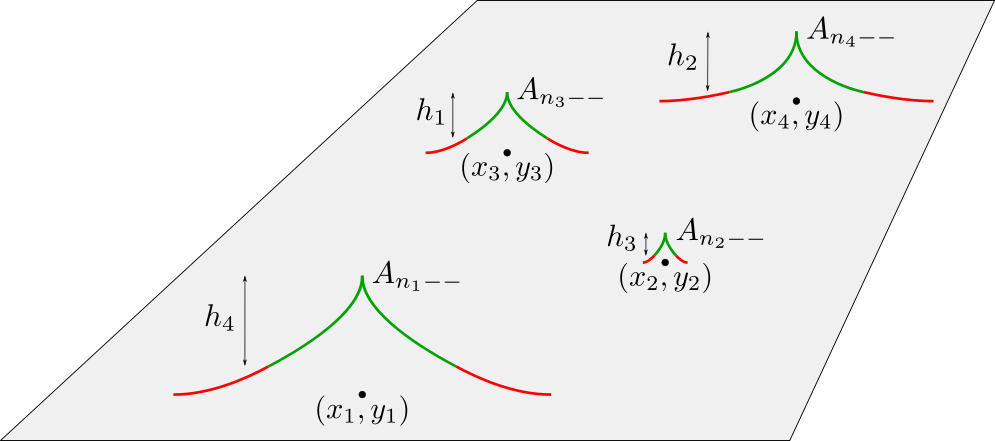
\includegraphics[scale=0.5]{images/img22}}
    \caption[Plane with singularities.]
    {Plane with singularities.}
    %id obrazku, pomocou ktoreho sa budeme na obrazok odvolavat
    \label{img:22}
\end{figure}
There are some limitations on the input data. As we do not want the singularities 
or the bump functions to intersect, we require that each pair of input points is
distanced $d_{ij}$ from each other. We specify the $d_{ij}$ value in the section~\ref{limitations}.
\subsubsection*{Bump function}
\begin{definition}
The support $supp(f)$ of a function $f: \R^n \to \R$ is a set of points where $f$ is not
zero $$supp(f) = \{ x\in \R^n : f(x)\neq 0 \}.$$
The closed support of the function $f$ is defined as a closure of $supp(f)$.
\end{definition}
Bump function if a function $f:\R^n \to \R$ which is smooth ($C^\infty$) and
compactly supported (the closed support of the function $f$ is a compact subset
of $\R^n$).

The most common example of such bump function is the function 
$$f(x)= \left\{
    \begin{array}{ll}
        e^{-\frac{1}{1-x^2}}, & x \in (-1, 1) \\
          0, & otherwise,\\
    \end{array} 
    \right. $$
which is both $C^\infty$ and compactly supported.

The bump function can smoothly connect a curve to a line or a surface to a
plane in a higher dimension. If we only need to connect a curve and a line $C^n$ smoothly, 
we only need a bump function which connects $C^n$ smoothly to a line.

In our work, we connect two surfaces with $C^1$ continuity and for this purpose
we use the function
$$f(x)= \left\{
    \begin{array}{ll}
        -q \cdot cos(k \cdot x)-q, & x \in (-\frac{\pi}{k}, \frac{\pi}{k}) \\
        0, & otherwise,\\
    \end{array} 
    \right. $$
rotated about $z$-axis.
The result of the rotation is the following function:
$$f(x, y) = \left\{
    \begin{array}{ll}
        -q \cdot cos(k \cdot (x^2+y^2))-q, & x^2+y^2<=(\frac{\pi}{k})^2 \\
        0, & otherwise.\\
    \end{array} 
    \right. $$
These functions can be seen in the Figure~\ref{img:21}.
\begin{figure}
    \centerline{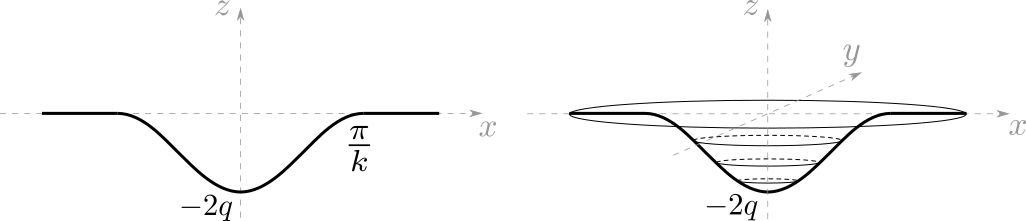
\includegraphics[scale=0.5]{images/img21}}
    \caption[$C^1$ cosine bump function.]
    {$C^1$ cosine bump function.}
    %id obrazku, pomocou ktoreho sa budeme na obrazok odvolavat
    \label{img:21}
\end{figure}

\subsubsection*{Implicit equation of the cosine bump function}
To construct the implicit equation of the cosine bump function, we use CSG
- constructive solid geometry, described in the section~\ref{sub2.6}.

First, we cut out the part of the rotated cosine, where
$x^2+y^2<(\frac{\pi}{k})^2$ using cylinder and intersection operation. Next,
we use a plane and the union operation to \textit{glue} the bump to the plane.
The described process is displayed in the Figure~\ref{img:24} in the form of a CSG tree.
\begin{figure}
    \centerline{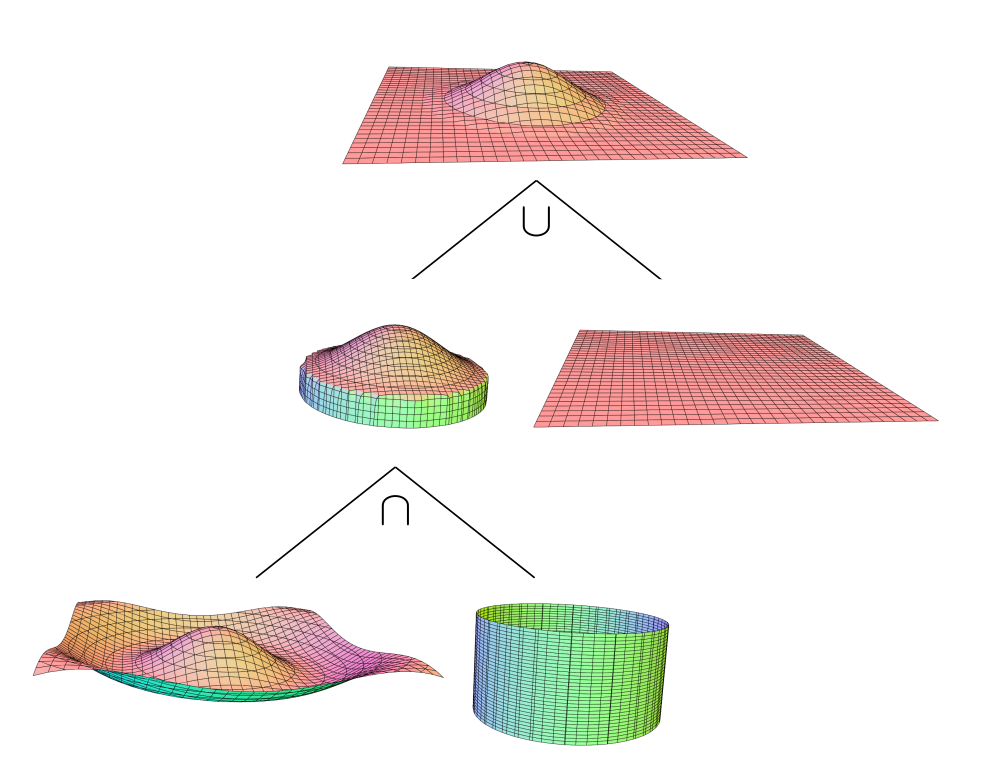
\includegraphics[scale=0.5]{images/img24}}
    \caption[Construction of the cosine bump function using CSG]
    {Construction of the cosine bump function using CSG \cite{calcplot3d}.}
    %id obrazku, pomocou ktoreho sa budeme na obrazok odvolavat
    \label{img:24}
\end{figure}
We use the following equations of the surfaces to model the cosine bump function:

\begin{table}[]
    \centering
    \begin{tabular}{|c|c|}
        \hline\hline
    Function name            & Implicit equation                                        \\ \hline\hline
    Rotated cosine function & $x+q \cdot cos(k \cdot \sqrt{(y-p_y)^2+(z-p_z)^2})+q=0$  \\ \hline
    Cylinder                & $(y-p_y)^2+(z-p_z)^2-(\frac{\pi}{k})^2=0$                \\ \hline
    Plane                   & x=0                                                      \\ \hline\hline
    \end{tabular}
    \caption[Implicit equations for bump function modelling]
    {Implicit equations for bump function modelling.}
    \label{tab:1}
    \end{table}

Parameters $q$ and $k$ allow us to change the amplitude and the frequency of
the cosine function, parameters $p_y$ and $p_z$ are used to move the bump function
to the given point $(p_y, p_z)$.

\subsubsection*{Attaching singularities to the plane using the cosine bump function}

Given the type of the singularity -- $n$ and given height -- $h$, we calculate the
constants of the cosine bump function to connect $C^1$ smoothly to the given
singularity.

The singularity given by the implicit equation $x^{n+1}-y^2-z^2$ intersected with 
the plane $x=h$ produces a circle with the radius $r=\sqrt{h^{n+1}}$.
The cosine bump function is scaled using $q$ and $k$ to smoothly connect the
singularity in the middle of the cosine bump function. This approach is displayed
in the Figure~\ref{img:25}. 

\begin{figure}
    \centerline{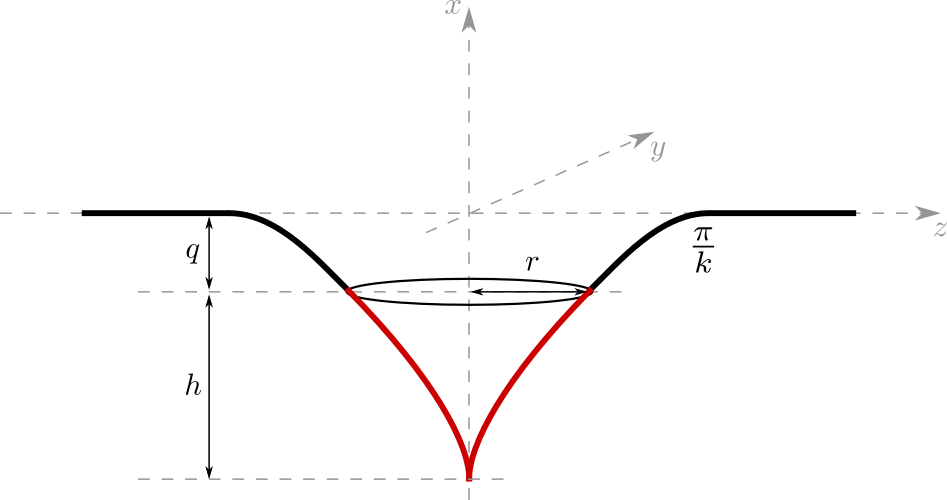
\includegraphics[scale=0.5]{images/img25}}
    \caption[Attaching the singularity to a plane using the cosine bump function]
    {Attaching the singularity to a plane using the cosine bump function.}
    %id obrazku, pomocou ktoreho sa budeme na obrazok odvolavat
    \label{img:25}
\end{figure}

As the singularity is attached in the middle of the
bump function, we get the equality $r=\frac{\pi}{2k}$ and therefore
$\sqrt{h^{n+1}}=\frac{\pi}{2k} \implies k=\pi/(2\sqrt{h^{n+1}})$.
The parameter $q$ is calculated from the $C^1$ continuity requirement. We require the
gradients to be linearly dependent on the points of connection. Due to the rotation
symmetry, we check it only for the intersection with the plane $z=0$
for the point $(-q, \frac{\pi}{2k})$.
$$F=(x+h+q)^{n+1}-y^2 \implies \nabla F = \left[(n+1)(x+h+q)^n, -2y\right]$$
$$\nabla F \left(-q, \frac{\pi}{2k}\right) = \left[(n+1) h^n, -\frac{\pi}{k}\right]$$
$$G=x+q \cdot cos(k y)+q \implies \nabla G = \left[1, -qk \cdot sin(k y)\right]$$
$$\nabla G \left(-q, \frac{\pi}{2k}\right) = \left[1, -qk \right]$$

Requiring $\nabla F (-q, \frac{\pi}{2k}) = s \cdot \nabla G (-q, \frac{\pi}{2k})$
and knowing $k=\pi/(2\sqrt{h^{n+1}})$, we get $s=(n+1)h^n$ and therefore $q=4h/(\pi(n+1))$.

After calculating the parameters $q$ and $k$ of the cosine bump function, 
we proceed to connect the singularity to the bump function.
We use intersection with the plane $x=-q$ to get the sections of the singularity
and the section of the bump function, and lastly, we use the union of these two 
surfaces. The described process is displayed in the Figure~\ref{img:26}.
The information about the detailed calculation of the implicit equation 
can be found in the appendix~\ref{appA}.

\begin{figure}
    \centerline{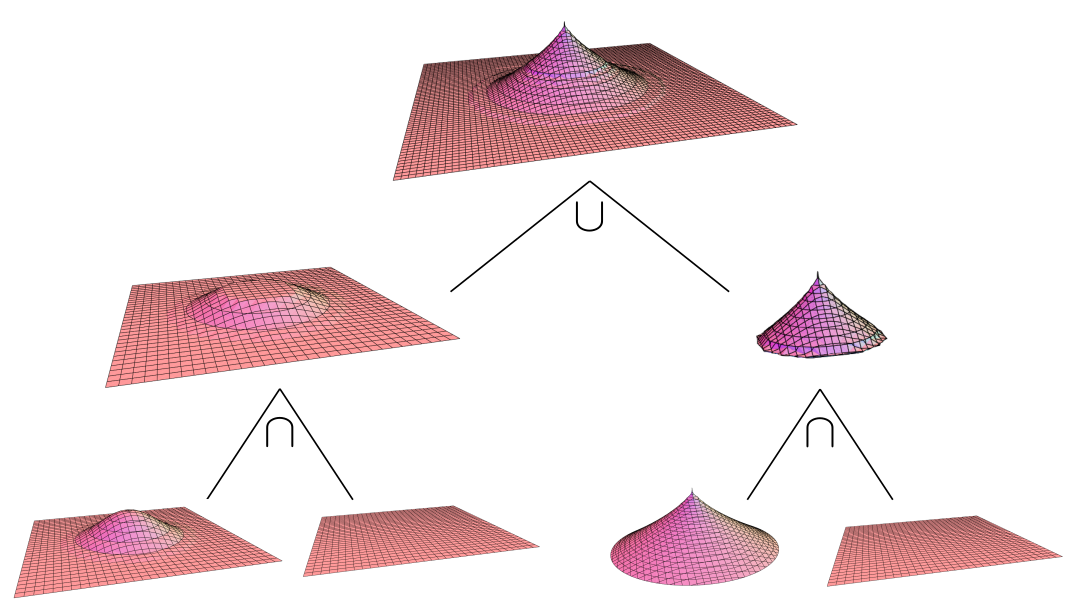
\includegraphics[scale=0.5]{images/img26}}
    \caption[Attaching the singularity to a plane using CSG]
    {Attaching the singularity to a plane using CSG \cite{calcplot3d}.}
    %id obrazku, pomocou ktoreho sa budeme na obrazok odvolavat
    \label{img:26}
\end{figure}

To connect multiple singularities to the same plane, we construct the implicit
equation for each singularity and then use the union operation to
create a surface with multiple singularities. This procedure is displayed in
the Figure~\ref{img:28}.

\begin{figure}
    \centerline{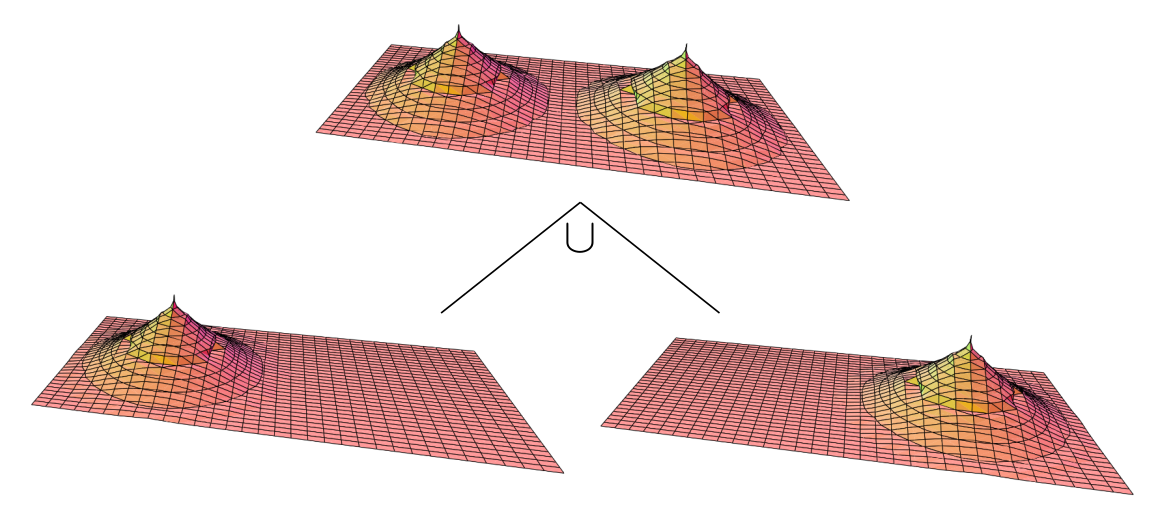
\includegraphics[scale=0.5]{images/img28}}
    \caption[Plane with multiple attached singularities]
    {Plane with multiple attached singularities \cite{calcplot3d}.}
    %id obrazku, pomocou ktoreho sa budeme na obrazok odvolavat
    \label{img:28}
\end{figure}

\subsubsection*{Limitations on the input data}
\label{limitations}
As mentioned, we require that each pair of input points is
distanced $d_{ij}$ from each other. As the radius of the closed support
of the cosine bump function is $r=\frac{\pi}{k}=2\sqrt{h^{n+1}}$, the 
distance between two input points $p_j, p_j$ must be at least
$d_{ij} = 2\sqrt{h_i^{n_i+1}}+2\sqrt{h_j^{n_j+1}}$. This way, both singularities
and the corresponding bump functions do not intersect. 

Let $l$ be the number of layers used for the triangulation and let $h_e$ be the height
calculated from the input edge length $e$ as shown in the chapter \ref{An--singularities}.
Then, the height $h$ displayed on the image \ref{img:25} must be bigger than the
height $h_e$.

\section{Triangulation of non-isolated singularities}
\label{sub3.3} 

We present an approach for triangulation of implicit surfaces with singular
curves which are
a result of performing intersection operation on the interiors of two
regular implicit surfaces.

We start by creating a local mesh for the surroundings of these singular
curves and finish the mesh in the regular parts.

\subsection{Creating the local mesh around the singular curves}

We start by approximating the singular curve by a polyline.
On the input, one point close to the singular curve is given. This point serves as
a starting point $P_0$. The tangent vector $\vec{t}_C(P_0)$ of the curve is computed as
the cross product of the unit normal vectors of the two surfaces $S_1$ and $S_2$ given
by the implicit equations $F_1=0$ and $F_2=0$, respectively.
Given the required approximate edge length $e$, a point $Q_1$ is computed as
$Q_1 = P_0 + e \cdot \vec{t}_C(P_0)$. We obtain the point $P_1$ by projecting the point 
$Q_1$ to the curve $C$ using an approach described in the section~\ref{sub2.3}.
Other points are then created iteratively by the same approach:
$$Q_{n+1} = P_n + e \cdot \vec{t}_C(P_n),$$
$$P_{n+1} = proj_C(Q_{n+1}),$$
while checking if the new point is inside the axis-aligned bounding box.
We stop once the new point is outside of the axis-aligned bounding box or
if the new point is close to the starting point $P_0$, which means the approximated
the curve is a closed curve.

In the case of the open curve, to complete the whole polyline, we also approximate 
the second part of the singular curve by iteratively creating points in the 
opposite direction, starting from point $P_0$. Let $m$ be the number of points
in the polyline the second part of the polyline consists of the points
$P_m, P_{m+1}, ...$, where
$$Q_m = P_0 - e \cdot \vec{t}_C(P_0),$$
$$P_m = proj_C(Q_m),$$
and again, iteratively
$$Q_{n+1} = P_n - e \cdot \vec{t}_C(P_{n}), \hspace{5mm} n = m, m+1, ...$$
$$P_{n+1} = proj_C(Q_{n+1}), \hspace{5mm} n = m, m+1, ...$$

The presented approach is visualized in two dimensions in the Figure~\ref{img:37}.

\begin{figure}
    \centerline{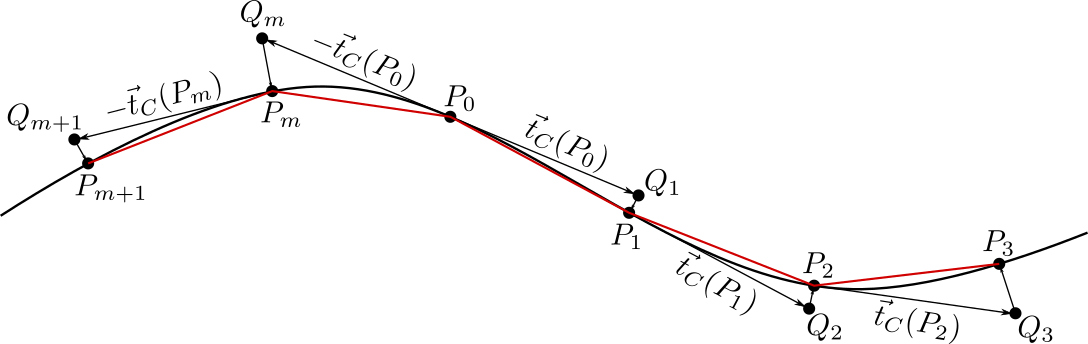
\includegraphics[scale=0.5]{images/img37}}
    \caption[Approximation of the implicit curve by polyline]
    {Approximation of the implicit curve by a polyline.}
    %id obrazku, pomocou ktoreho sa budeme na obrazok odvolavat
    \label{img:37}
\end{figure}

After obtaining the polyline approximation of the curve on the intersection
of the two surfaces, one may create the local mesh. Let us rename the polyline 
points to $P_0, P_1, ..., P_k$, such that $l_i = \overline{P_i P_{i+1}}$ is a 
line segment of the polyline for $i=0, ..., k-1$ (and $l_k = \overline{P_k P_0}$ is a 
a line segment of the polyline for a closed curve).

For each line segment $l_i$, we create two adjacent triangles containing $l_i$.

We start by calculating the midpoint $M_i = \frac{P_i+P_{i+1}}{2}$.
By projecting the point $M_i$ to the surface $S_1$, we obtain the point $M_i^1$.
By projecting it to the surface $S_2$, we obtain the point $M_i^2$. The defined points
are visualized in the Figure~\ref{img:38}.

\begin{figure}[h!]
    \centerline{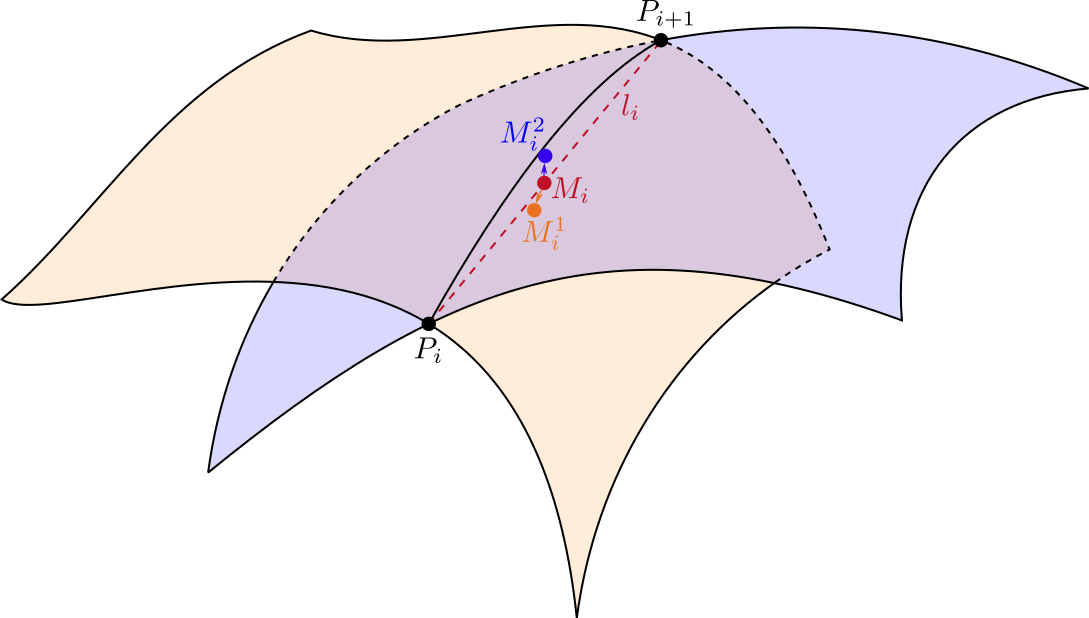
\includegraphics[scale=0.5]{images/img38}}
    \caption[Definition of the points]
    {Definition of the points $M_i$, $M_i^1$ and $M_i^2$.}
    %id obrazku, pomocou ktoreho sa budeme na obrazok odvolavat
    \label{img:38}
\end{figure}

As the point $M_i^1$ is lying on the surface, the tangent plane $T_{S_1}(M_i^1)$ 
of the surface $S_1$ in the point $M_i^1$ is well defined. The same holds for the 
point $M_i^2$ lying on the surface $S_2$. 

We first define points $R_i^1$ and $R_i^2$ close to the surface. After projecting
these points on the surface, we obtain the third point for each of the two 
adjacent triangles.

The point $R_i^1$ is obtained by moving from the point $M_i$ in the direction 
perpendicular to both $\overrightarrow{P_{i} P_{i+1}}$ and 
$\nabla{F_1}(M_1)$ by the given edge length $e$.

$$R_i^1 = M_i + e \cdot \frac{\nabla{F_1}(M_1) \times \overrightarrow{P_{i} P_{i+1}}}{||\nabla{F_1}(M_1) \times \overrightarrow{P_i P_{i+1}}||}.$$

The described situation is displayed in the Figure~\ref{img:39}.
For the point $M_i$, the plane $H_i$ passing through $M_i$, perpendicular to the
line segment $l_i$ is defined:
$$H_i : \overrightarrow{P_i P_{i+1}} \cdot (X-M_i) = 0.$$
For better understanding, the Figure~\ref{img:39} is the projection of the surroundings
of the point $M_i$ to the plane $H_i$. Generally, points $M_i^1$ and $M_i^2$ do not lie in
the plane $H_i$. The points $R_i^1$ and $R_i^2$ are picked in such way, that the point
$R_i^1$ does not lie outside of the $S_2$ and the point $R_i^2$ does not lie outside of 
the surface $S_1$.

\begin{figure}[h!]
    \centerline{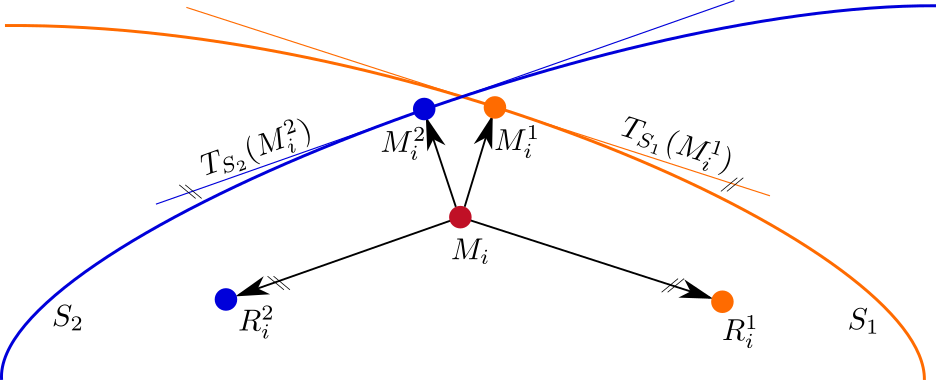
\includegraphics[scale=0.5]{images/img39}}
    \caption[Definition of the points]
    {Definition of the points $R_i^1$ and $R_i^2$ in the plane $H_i$.}
    %id obrazku, pomocou ktoreho sa budeme na obrazok odvolavat
    \label{img:39}
\end{figure}

The points $R_i^1$ and $R_i^2$ are projected to the surface given by the intersection
of the interiors of the two surfaces. The equation defining the surface is 
$$F_{1 \cap 2} = F_1 + F_2 + \sqrt{F_1^2+F_2^2}.$$

An example of the resulting local mesh for an open curve is displayed in the image
\ref{img:local-mesh-sing-curve}. This curve is a part of the singular curve on the surface 
given by the intersection of the interiors of a sphere and a hyperboloid.

\begin{figure}[h!]
    \centerline{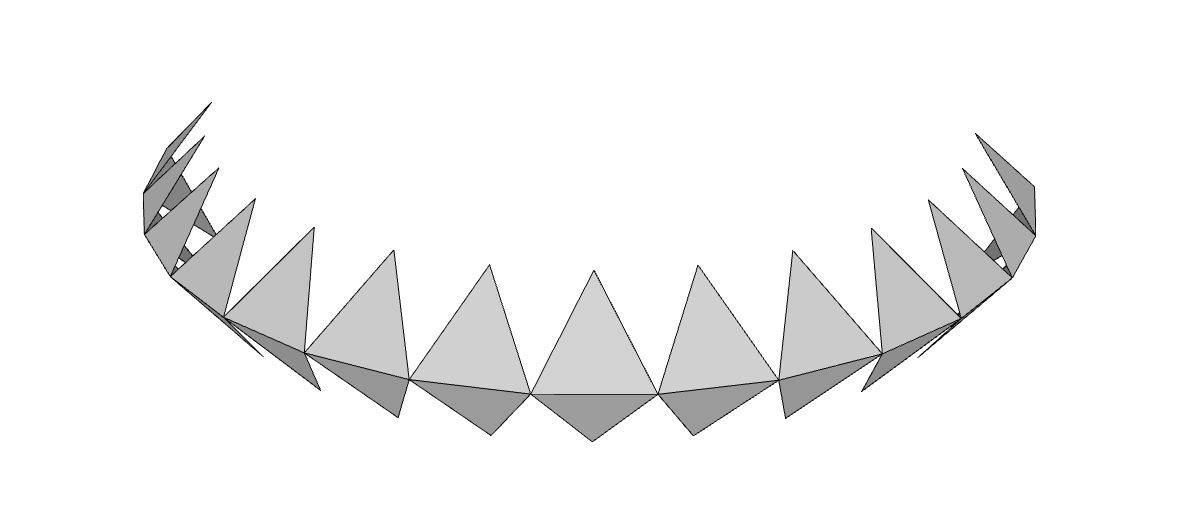
\includegraphics[scale=0.3]{images/local-mesh-sing-curve}}
    \caption[Local mesh around the singular curve]
    {Local mesh around the singular curve.}
    %id obrazku, pomocou ktoreho sa budeme na obrazok odvolavat
    \label{img:local-mesh-sing-curve}
\end{figure}

\subsection{Modification for triangulation of the union and the difference}
For the intersection, the points $R_i^1$ and $R_i^2$ were picked in such way, that the point
$R_i^1$ does not lie outside of the $S_2$ and the point $R_i^2$ does not lie outside of 
the surface $S_1$. The local mesh for the union is achieved by picking $R_i^1$ and $R_i^2$
in such way, that $R_i^1$ does not lie inside of $S_2$ and the point $R_i^2$ does not lie 
inside of the surface $S_1$. The points $R_i^1$ and $R_i^2$ for creating local mesh for 
the union of the interiors is displayed on the Figure~\ref{img:75}.

\begin{figure}[h!]
    \centerline{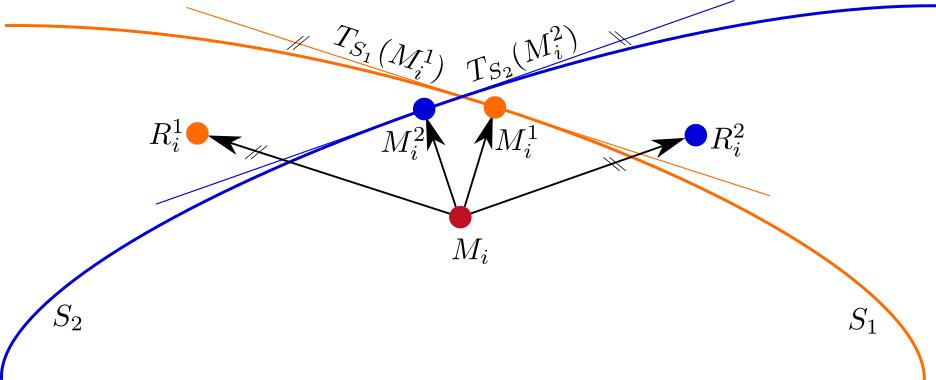
\includegraphics[scale=0.5]{images/img75}}
    \caption[Definition of the points for union]
    {Definition of the points $M_i$, $M_i^1$ and $M_i^2$ for union.}
    %id obrazku, pomocou ktoreho sa budeme na obrazok odvolavat
    \label{img:75}
\end{figure}

For the difference, the points $R_i^1$ and $R_i^2$ are picked in such way, that $R_i^1$ 
does not lie inside of $S_2$ and the point $R_i^2$ does not lie 
outside of the surface $S_1$. The points $R_i^1$ and $R_i^2$ for creating local mesh for 
the difference of the interiors is displayed on the Figure~\ref{img:75}.

\begin{figure}[h!]
    \centerline{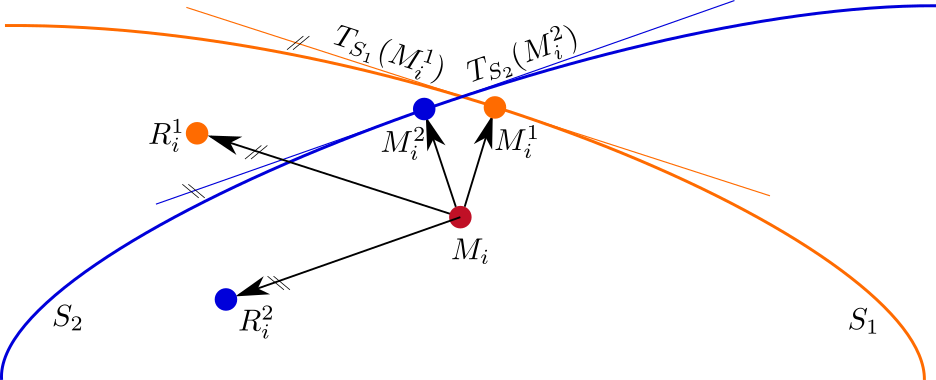
\includegraphics[scale=0.5]{images/img76}}
    \caption[Definition of the points for difference]
    {Definition of the points $M_i$, $M_i^1$ and $M_i^2$ for difference.}
    %id obrazku, pomocou ktoreho sa budeme na obrazok odvolavat
    \label{img:76}
\end{figure}
